%%-----------------------------------------------------------------------
%% IEEE Conference Paper -- Power Quality Disturbance Classification
%% Two-Stage Threshold + Hybrid 1D-CNN + Random Forest pipeline
%% with IEEE 1159 Knowledge-Based Severity Reasoning.
%%
%% Compile order on Overleaf (use pdfLaTeX):
%%   1. pdflatex main
%%   2. bibtex   main
%%   3. pdflatex main
%%   4. pdflatex main
%%-----------------------------------------------------------------------

\documentclass[conference]{IEEEtran}
\IEEEoverridecommandlockouts

\usepackage{cite}
\usepackage{amsmath,amssymb,amsfonts}
\usepackage{algorithm}
\usepackage{algpseudocode}
\usepackage{graphicx}
\usepackage{textcomp}
\usepackage{xcolor}
\usepackage{booktabs}
\usepackage{array}
\usepackage{multirow}
\usepackage{tikz}
\usetikzlibrary{shapes.geometric, arrows.meta, positioning, calc, fit}
\usepackage{url}
\usepackage{hyperref}
\hypersetup{
  colorlinks=true,
  linkcolor=black,
  citecolor=black,
  urlcolor=blue
}

\newcolumntype{C}[1]{>{\centering\arraybackslash}p{#1}}
\newcolumntype{R}[1]{>{\raggedleft\arraybackslash}p{#1}}

\def\BibTeX{{\rm B\kern-.05em{\sc i\kern-.025em b}\kern-.08em
    T\kern-.1667em\lower.7ex\hbox{E}\kern-.125emX}}

\title{A Two-Stage Hybrid Convolutional Neural Network and Random Forest
Pipeline for Real-Time Power Quality Disturbance Classification with
Knowledge-Based Severity Reasoning}

\author{
\IEEEauthorblockN{Shrimathi G}
\IEEEauthorblockA{Department of Electrical and\\
Electronics Engineering\\
Sri Venkateswara College of Engineering\\
Pennalur 602117\\
2022ee0135@svce.ac.in}
\and
\IEEEauthorblockN{Sanjay Kumar V}
\IEEEauthorblockA{Department of Electrical and\\
Electronics Engineering\\
Sri Venkateswara College of Engineering\\
Pennalur 602117\\
2022ee0214@svce.ac.in}
\and
\IEEEauthorblockN{Suresh N}
\IEEEauthorblockA{Department of Electrical and\\
Electronics Engineering\\
Sri Venkateswara College of Engineering\\
Pennalur 602117\\
sureshn@svce.ac.in}
}

\begin{document}
\maketitle

% --- Abstract ----------------------------------------------------------
\begin{abstract}
This paper presents a two-stage hybrid pipeline for real-time
classification of power quality disturbances (PQDs) defined under
IEEE~Standard~1159. The proposed system processes raw single-cycle
voltage windows of 100 samples acquired at 5~kHz, corresponding to one
period of the 50~Hz fundamental. Stage~1 implements an $O(N)$
rule-based threshold detector that operates on five physical features ---
root mean square, low-order total harmonic distortion, excess kurtosis,
maximum consecutive-sample difference, and quarter-window root mean
square dispersion --- and produces a binary Normal/Abnormal decision in
less than one millisecond. Windows flagged as Abnormal are escalated to
Stage~2, a hybrid classifier in which a compact one-dimensional
convolutional neural network learns a 64-dimensional feature
representation directly from the raw waveform, and a Random Forest with
200 decision trees performs the final classification across seventeen
classes (one normal type, eight single disturbances, and eight pairwise
compound disturbances). Each classified window is enriched at run time
with a severity grade, probable cause, equipment-at-risk, and three to
five recommended operator actions retrieved from a 17-entry knowledge
base derived from IEEE~Standard~1159, and the result is streamed to a
browser dashboard through a Flask-SocketIO backend. Evaluation on a
stratified 80-to-20 split of the 17{,}000-signal XPQRS dataset
(3{,}400 held-out signals) yields a Stage~2 classification accuracy of
98.85\%, with thirteen of seventeen classes attaining 100\% recall, an
end-to-end pipeline accuracy of 96.67\% on a balanced mixed-traffic
test, a 100\% Normal-detection rate at zero false alarms in Stage~1,
and a complete-path inference latency of approximately 67~milliseconds
on a single-thread laptop CPU without graphics-processing-unit
acceleration or cloud connectivity. A preprocessing analysis further
demonstrates that per-sample maximum-absolute normalization, frequently
adopted in the deep-learning PQD literature, reduces classification
accuracy to 52\% by discarding the amplitude information that
distinguishes Sag, Swell, and Interruption from Pure Sinusoidal; a
single global-scale normalization derived from the training distribution
restores the missing 47 percentage points. Post-hoc SHAP attribution is
integrated on the legacy feature-based baseline to support
operator-side review of borderline predictions. The proposed system
satisfies the operational latency constraint imposed by one-cycle
decision deadlines and is therefore suitable for edge deployment on
distribution feeders.
\end{abstract}

\begin{IEEEkeywords}
Power quality, power quality disturbance classification,
IEEE~Standard~1159, two-stage pipeline, one-dimensional convolutional
neural network, random forest, hybrid classifier, real-time monitoring,
edge intelligence, knowledge-based reasoning, SHAP interpretability.
\end{IEEEkeywords}

% =====================================================================
\section{Introduction}
% =====================================================================
Power quality (PQ) has emerged as a critical concern in contemporary
power systems owing to the increasing penetration of renewable energy
resources, power-electronic converters, electric-vehicle charging
infrastructure, and non-linear industrial loads. The injection of
non-sinusoidal currents into distribution networks produces voltage
waveforms whose deviation from the nominal sinusoid is frequently the
limiting factor for sensitive end-use equipment. The categorization of
such deviations --- voltage sag, voltage swell, interruption, harmonic
distortion, flicker, impulsive transient, oscillatory transient,
notching, and their pairwise compound combinations --- is formally
defined in IEEE~Standard~1159~\cite{ieee1159}. A deployable PQ monitor
is required to identify the specific disturbance class within an
operationally relevant time window~\cite{khetarpal2020review,
mahela2021review}.

Conventional PQ classification approaches extract handcrafted
statistical or spectral features (root mean square, total harmonic
distortion, wavelet energies, higher-order statistics) from each
waveform window and apply a shallow classifier such as a support
vector machine, an extreme learning machine, or a decision-tree
ensemble~\cite{thirumala2020classification, sahani2021rf,
chakravorti2021ensemble}. Recent literature has demonstrated that
one-dimensional convolutional neural networks (1D-CNNs)~\cite{wang2021hybrid,
cai2020wigner, eristi2022realtime} can achieve competitive
classification accuracy directly from the raw voltage cycle without
explicit feature engineering. Hybrid configurations~\cite{cai2021hybrid,
liu2020curvelet, garcia2022edge}, in which a CNN serves as a learned
feature extractor followed by a classical classifier, represent an
active line of investigation aimed at obtaining the representational
capacity of deep models while retaining the deployment characteristics
of classical methods.

This paper presents a real-time PQ classification system that
integrates these two paradigms within a unified two-stage architecture
and contributes three system-level components that, to the best of the
authors' knowledge, have not been reported together in a single
published pipeline. First, a five-feature $O(N)$ rule-based screen
serves as Stage~1 and resolves clean traffic in less than one
millisecond, restricting the heavier classifier to flagged windows.
Second, a hybrid 1D-CNN and Random Forest classifier serves as Stage~2
and performs 17-class classification on the windows escalated by
Stage~1. Third, an IEEE~1159-derived knowledge base augments every
classified output with a severity grade, physical cause, equipment-at-risk,
and three to five immediate operator actions. The full pipeline executes
on a single-thread laptop-class CPU without graphics-processing-unit
(GPU) acceleration or external network connectivity, and is shown to
satisfy operational latency requirements that cloud-deployed deep PQ
classifiers cannot meet under typical wide-area round-trip-time
constraints~\cite{xiao2023iot}.

The remainder of the paper is organized as follows.
Section~\ref{sec:related} reviews related work.
Section~\ref{sec:problem} formalizes the problem statement, summarizes
the contributions, and articulates the novelties.
Section~\ref{sec:dataset} describes the dataset and the underlying
signal model. Section~\ref{sec:method} details the proposed methodology
and the supporting mathematical formulation. Section~\ref{sec:realtime}
describes the real-time backend and the dashboard.
Section~\ref{sec:exp} presents the experimental setup.
Section~\ref{sec:cmp} reports the model-selection comparison.
Section~\ref{sec:results} presents results and discussion.
Section~\ref{sec:limits} enumerates the limitations of the present
study, and Section~\ref{sec:conclusion} concludes the paper.

% =====================================================================
\section{Related Work}\label{sec:related}
% =====================================================================
PQ disturbance classification has been studied extensively. Khetarpal
and Tripathi~\cite{khetarpal2020review} provide a comprehensive review
of the field, surveying signal-processing, machine-learning, and hybrid
approaches and identifying the trade-offs between feature-engineering
depth and classification accuracy. Mahela \emph{et al.}\
\cite{mahela2021review} examine PQ assessment in distribution networks
with renewable penetration, employing a Stockwell-transform-based
detector with fuzzy clustering. Thirumala \emph{et al.}\
\cite{thirumala2020classification} apply empirical wavelet
transform-based adaptive filtering with a multiclass support vector
machine. Sahani and Dash~\cite{sahani2021rf} introduce a weighted
bidirectional extreme learning machine in conjunction with the
Hilbert--Huang transform. Chakravorti \emph{et al.}\
\cite{chakravorti2021ensemble} address PQ classification in microgrid
environments using hybrid signal-processing and machine-learning
techniques.

Deep-learning approaches have been investigated more recently. Wang
\emph{et al.}\ \cite{wang2021hybrid} employ a deep convolutional neural
network on compressed-sensing reconstructions of voltage cycles. Cai
\emph{et al.}\ \cite{cai2020wigner} feed Wigner--Ville distribution
images to a deep CNN. Eristi \emph{et al.}\ \cite{eristi2022realtime}
combine a one-dimensional local binary pattern operator with a CNN.
Garcia \emph{et al.}\ \cite{garcia2022edge} perform a comparative study
of CNN, long short-term memory, and CNN-LSTM architectures applied to
the same PQ disturbance set. Rodriguez-Guerrero \emph{et al.}\
\cite{rodriguez2022cnn} report parameter estimation of a parameterized
PQ disturbance model using metaheuristic optimization. The principal
trade-off across these systems is model size: typical published deep PQ
classifiers carry between $10^{5}$ and $10^{6}$ parameters, which is
acceptable for server-side execution but is unsuitable for embedded
deployment.

The work most closely related to the present study is that of Cai
\emph{et al.}\ \cite{cai2021hybrid}, which integrates a CNN feature
extractor with an extreme gradient boosting classifier for PQ
disturbance recognition. The present work adopts the broader hybrid
template --- a CNN feature extractor combined with an ensemble
classifier head --- and extends it along three axes: (i) the
introduction of an $O(N)$ rule-based screening stage that precedes the
heavier model; (ii) the extension of the class set to seventeen,
including eight pairwise compound disturbances; and (iii) the
integration of a deterministic IEEE~1159-grounded knowledge base that
emits severity, cause, equipment-at-risk, and immediate-action metadata
for every classified window.

Two-stage architectures that screen with a fast rule and invoke a
heavier model only on suspicious windows are common in time-series
anomaly detection in general~\cite{xiao2023iot}. However, no published
PQ system known to the authors has reported the screen behaviour with
both detection rate and false-alarm rate, employed a hybrid CNN and
tree-ensemble classifier as the second stage, and emitted
operator-actionable knowledge-base metadata as part of the deployed
pipeline.

Interpretability of PQ classifiers has historically received limited
attention. The TreeSHAP attribution method of Lundberg \emph{et al.}\
\cite{lundberg2020trees} enables tractable per-prediction attribution
for tree-based models, and is applied in the present work as a
post-hoc explainer on the legacy 36-feature Random Forest baseline.
Broader surveys of explainable artificial intelligence are provided in
\cite{linardatos2021xai}.

% =====================================================================
\section{Problem Statement, Contributions, and Novelties}
\label{sec:problem}
% =====================================================================
\subsection{Problem Statement}
Modern power systems are increasingly subject to PQ disturbances
arising from the proliferation of renewable energy sources,
power-electronic converters, and non-linear loads. These disturbances
introduce non-stationary and non-linear characteristics into the
voltage waveform, and their reliable identification under realistic
noise conditions remains technically demanding. Three constraints
define the operational solution space.

\subsubsection{Latency} A real-time PQ classifier must complete
inference within an operationally meaningful time-scale; for monitoring
and diagnostic applications this is one to a few cycles of the
fundamental.

\subsubsection{Class confusability} Several IEEE~1159 classes differ
from the normal reference solely in amplitude (sag, swell,
interruption), and several others are pairwise compounds of two single
disturbances. Both characteristics challenge feature- and
representation-learning methods.

\subsubsection{Deployability} A significant fraction of the published
deep-learning PQ literature presupposes cloud or GPU compute, which is
incompatible with edge-relay or substation-class hardware. Cloud
deployment further introduces a network round-trip-time penalty that
conventional links cannot absorb within a one-cycle decision deadline.

A classifier is therefore required that simultaneously (a) achieves
high accuracy across a large class set, (b) sustains low single-thread
CPU latency, (c) provides per-prediction interpretability, (d) emits
an output more actionable than a bare class label, and (e) operates
without external infrastructure.

\subsection{Contributions}
The principal contributions of this work are as follows.
\begin{enumerate}
  \item A two-stage classification pipeline comprising a
        five-feature $O(N)$ threshold screen as Stage~1 and a hybrid
        1D-CNN and Random Forest classifier as Stage~2.
  \item A hybrid CNN-RF classifier that achieves 98.85\% accuracy
        across seventeen IEEE~1159 classes, with thirteen of seventeen
        classes at 100\% recall.
  \item A knowledge-based output layer that augments every prediction
        with severity, cause, equipment-at-risk, and immediate-action
        metadata derived from IEEE~Standard~1159.
  \item A real-time backend and browser dashboard that streams
        predictions to all connected clients with sub-cycle Stage~1
        detection and approximately three-cycle Stage~2 classification
        on a laptop-class CPU.
  \item An input-normalization analysis that documents and explains a
        47-percentage-point accuracy collapse caused by per-sample
        maximum-absolute scaling, together with a single-line
        global-scale fix.
  \item A post-hoc SHAP explainer applied to the legacy 36-feature
        Random Forest baseline, returning the top three contributing
        physical features for any single prediction.
\end{enumerate}

\subsection{Novelties}\label{sec:novelties}
The novelties of the proposed system, taken together, define an
integrated pipeline whose combination of features has not been reported
in prior PQ literature.

\paragraph{N1. Two-stage architecture with rule-based screening and
hybrid deep classification}
The majority of published PQ classifiers operate as single-stage
end-to-end models. The proposed system introduces a five-feature
$O(N)$ rule-based screen that resolves the clean fraction of traffic in
under one millisecond and reserves the heavier hybrid model for windows
that cannot be classified at the rule level. The screen is
characterized by both a 100\% detection rate and a 0\% false-alarm
rate, a combination not jointly reported in prior PQ literature.

\paragraph{N2. Hybrid 1D-CNN and Random Forest with frozen-feature
retuning}
The 1D-CNN learns a 64-dimensional representation directly from the
raw cycle, and the Random Forest classifies on this representation.
The hybrid arrangement combines deep representational learning with
the calibrated top-$K$ probability outputs of a tree ensemble, and
permits the Random Forest head to be re-tuned on the frozen feature
space within seconds, without re-training the CNN.

\paragraph{N3. Knowledge-based severity-aware output layer}
Every prediction is enriched at inference time with a severity grade,
two-sentence physical cause, equipment-at-risk, and three to five
operator-level actions, drawn from a 17-entry knowledge base derived
from IEEE~Standard~1159. No prior PQ classifier known to the authors
emits this level of actionable diagnosis as part of the deployed
pipeline.

\paragraph{N4. Seventeen-class coverage including eight pairwise
compound disturbances}
The proposed system extends the class set beyond the typical nine to
fourteen classes covered in prior deep PQ classifiers, and demonstrates
thirteen of seventeen classes at 100\% recall.

\paragraph{N5. Global-scale normalization for amplitude-preserving
deep learning on PQ signals}
A 47-percentage-point accuracy collapse caused by the per-sample
maximum-absolute scaling commonly employed in the deep-learning PQ
literature is documented, and a single-line global-scale normalization
that restores the missing accuracy is presented. The result is
transferable to any deep PQ pipeline that includes
amplitude-distinguished classes.

\paragraph{N6. Real-time multi-source backend and offline-tolerant
dashboard}
The Flask-SocketIO and TCP backend ingests live signals from MATLAB,
Python, and JSON-over-HTTP senders concurrently, and pushes
predictions to a single-file browser dashboard with severity-coded
panels, top-three confidence display, latency timeline, and an offline
demo-mode fallback. The complete system executes on a laptop-class
CPU without GPU acceleration or cloud connectivity.

\paragraph{N7. Edge-deployable inference profile within the cloud
round-trip-time floor}
Stage~1 detection is completed in less than one millisecond, and
Stage~2 classification in approximately three cycles of the 50~Hz
fundamental. Wide-area cloud round-trip times are typically
100--300~ms before any inference is initiated~\cite{xiao2023iot}, which
is several multiples of one PQ cycle. The proposed system therefore
satisfies an operational deadline that cloud-deployed deep PQ
classifiers cannot satisfy under realistic network conditions.

\paragraph{N8. Post-hoc SHAP attribution with physical-feature
semantics}
A TreeSHAP explainer is integrated on the legacy 36-feature Random
Forest baseline, returning the top three contributing physical
features (root mean square, total harmonic distortion, harmonic
magnitudes, wavelet energies) for any single prediction. Operators are
therefore able to review borderline classifications using named
physical quantities rather than abstract activation maps.

% =====================================================================
\section{Dataset and Signal Model}\label{sec:dataset}
% =====================================================================
Each input to the proposed system is a one-cycle voltage window of
length $N = 100$ samples acquired at a sampling rate $f_s = 5$~kHz,
corresponding to one period of the 50~Hz fundamental. Amplitudes are
expressed in per-unit (pu) with the nominal peak value normalized to
1.0. The underlying signal-generation model conforms to the disturbance
definitions of IEEE~Standard~1159~\cite{ieee1159}. The publicly
available XPQRS-style synthetic dataset is employed for training and
evaluation. The dataset comprises 17{,}000 signals balanced across
seventeen classes (1{,}000 signals per class). The seventeen classes
are: Pure Sinusoidal (the normal reference), voltage sag, voltage
swell, interruption, impulsive transient, oscillatory transient,
harmonics, notch, flicker, and eight pairwise compound disturbances
formed by combinations of sag, swell, harmonics, flicker, oscillatory
transient, and notch.

Additive white Gaussian noise (AWGN) at a signal-to-noise ratio of
40~dB is applied during training to discourage memorization of
artefacts of the synthetic generator. A stratified 80-to-20 split with
random seed 42 is used, yielding 13{,}600 training samples and
3{,}400 test samples (200 per class).

The signal characteristics merit explicit description. A pure sinusoid
is a unit-amplitude sine wave at 50~Hz. A voltage sag corresponds to
multiplication of the sinusoid by a constant in the range
$0.1$--$0.9$~pu over a stretch of cycles, while a voltage swell
corresponds to multiplication by a constant in the range
$1.1$--$1.8$~pu. An interruption is approximated by a near-zero
amplitude window. Harmonic disturbances superimpose integer-multiple
sinusoids on the fundamental. Flicker corresponds to slow amplitude
modulation of the fundamental. Several classes --- sag, swell, and
interruption --- therefore differ from the normal reference solely in
amplitude. As demonstrated in Section~\ref{sec:results}, this
characteristic interacts critically with the choice of input
normalization.

% =====================================================================
\section{Methodology}\label{sec:method}
% =====================================================================
\subsection{System Overview}
The proposed framework follows a structured pipeline: signal
acquisition, preprocessing, two-stage classification, knowledge-base
enrichment, and real-time push to the dashboard.
Fig.~\ref{fig:arch} illustrates the overall architecture. A signal
arrives via TCP, HTTP, or a SocketIO event. Stage~1 produces a binary
Normal/Abnormal decision in under one millisecond. If the decision is
Normal, the prediction is reported as Pure Sinusoidal and the call
returns. If the decision is Abnormal, the same window is forwarded to
Stage~2, which produces a 17-class label and a confidence vector. The
result is enriched with knowledge-base metadata and pushed to all
connected dashboard clients.

\begin{figure*}[t]
  \centering
  % Two-stage architecture diagram (TikZ).
% Used in main.tex as:  % Two-stage architecture diagram (TikZ).
% Used in main.tex as:  % Two-stage architecture diagram (TikZ).
% Used in main.tex as:  \input{figures/architecture}
% Sized to fit a two-column IEEE figure* (max ~17.6cm).

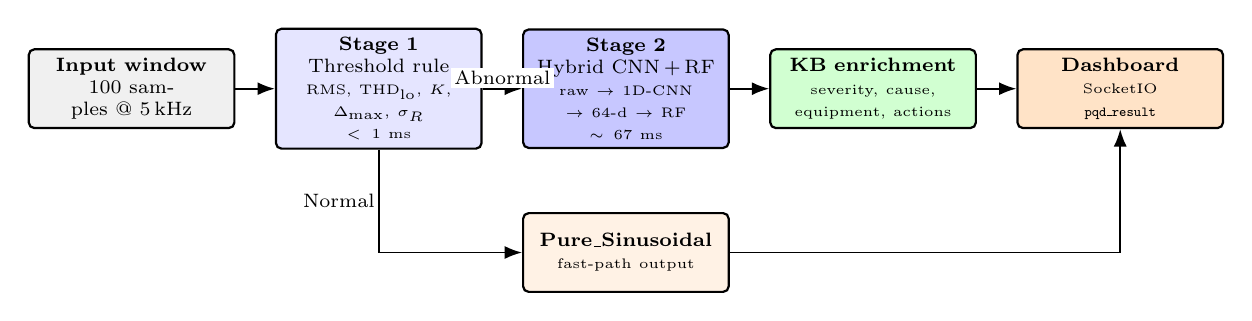
\begin{tikzpicture}[
  font=\scriptsize,
  align=center,
  every path/.style={-{Latex[length=2.2mm]}, thick, line width=0.6pt},
  blk/.style={rectangle, rounded corners=2pt, draw=black, thick,
              minimum height=10mm, text width=2.4cm, inner sep=3pt},
  io/.style={blk, fill=gray!12},
  s1/.style={blk, fill=blue!10},
  s2/.style={blk, fill=blue!22},
  kb/.style={blk, fill=green!18},
  dst/.style={blk, fill=orange!22},
  fast/.style={blk, fill=orange!10, text width=2.4cm},
  lbl/.style={font=\scriptsize, inner sep=1.2pt, fill=white},
]

\node[io]                       (in)   {\textbf{Input window}\\
                                        100 samples @ 5\,kHz};
\node[s1, right=5mm of in]      (st1)  {\textbf{Stage 1}\\Threshold rule\\
                                        {\tiny RMS, THD$_{\mathrm{lo}}$, $K$,}\\
                                        {\tiny $\Delta_{\max}$, $\sigma_R$}\\
                                        {\tiny $<\!1$ ms}};
\node[s2, right=5mm of st1]     (st2)  {\textbf{Stage 2}\\Hybrid CNN\,+\,RF\\
                                        {\tiny raw $\to$ 1D-CNN}\\
                                        {\tiny $\to$ 64-d $\to$ RF}\\
                                        {\tiny $\sim\!67$ ms}};
\node[kb, right=5mm of st2]     (kb)   {\textbf{KB enrichment}\\
                                        {\tiny severity, cause,}\\
                                        {\tiny equipment, actions}};
\node[dst, right=5mm of kb]     (push) {\textbf{Dashboard}\\
                                        {\tiny SocketIO}\\
                                        {\tiny \texttt{pqd\_result}}};

\node[fast, below=8mm of st2]   (norm) {\textbf{Pure\_Sinusoidal}\\
                                        {\tiny fast-path output}};

\draw (in)  -- (st1);
\draw (st1) -- node[lbl, above]{Abnormal} (st2);
\draw (st2) -- (kb);
\draw (kb)  -- (push);

\draw (st1.south) |- node[lbl, near start, left]{Normal} (norm.west);
\draw (norm.east) -| (push.south);

\end{tikzpicture}

% Sized to fit a two-column IEEE figure* (max ~17.6cm).

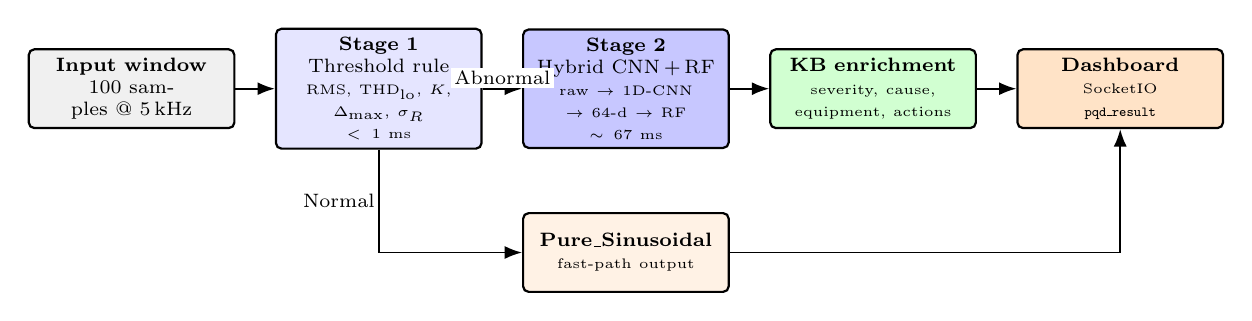
\begin{tikzpicture}[
  font=\scriptsize,
  align=center,
  every path/.style={-{Latex[length=2.2mm]}, thick, line width=0.6pt},
  blk/.style={rectangle, rounded corners=2pt, draw=black, thick,
              minimum height=10mm, text width=2.4cm, inner sep=3pt},
  io/.style={blk, fill=gray!12},
  s1/.style={blk, fill=blue!10},
  s2/.style={blk, fill=blue!22},
  kb/.style={blk, fill=green!18},
  dst/.style={blk, fill=orange!22},
  fast/.style={blk, fill=orange!10, text width=2.4cm},
  lbl/.style={font=\scriptsize, inner sep=1.2pt, fill=white},
]

\node[io]                       (in)   {\textbf{Input window}\\
                                        100 samples @ 5\,kHz};
\node[s1, right=5mm of in]      (st1)  {\textbf{Stage 1}\\Threshold rule\\
                                        {\tiny RMS, THD$_{\mathrm{lo}}$, $K$,}\\
                                        {\tiny $\Delta_{\max}$, $\sigma_R$}\\
                                        {\tiny $<\!1$ ms}};
\node[s2, right=5mm of st1]     (st2)  {\textbf{Stage 2}\\Hybrid CNN\,+\,RF\\
                                        {\tiny raw $\to$ 1D-CNN}\\
                                        {\tiny $\to$ 64-d $\to$ RF}\\
                                        {\tiny $\sim\!67$ ms}};
\node[kb, right=5mm of st2]     (kb)   {\textbf{KB enrichment}\\
                                        {\tiny severity, cause,}\\
                                        {\tiny equipment, actions}};
\node[dst, right=5mm of kb]     (push) {\textbf{Dashboard}\\
                                        {\tiny SocketIO}\\
                                        {\tiny \texttt{pqd\_result}}};

\node[fast, below=8mm of st2]   (norm) {\textbf{Pure\_Sinusoidal}\\
                                        {\tiny fast-path output}};

\draw (in)  -- (st1);
\draw (st1) -- node[lbl, above]{Abnormal} (st2);
\draw (st2) -- (kb);
\draw (kb)  -- (push);

\draw (st1.south) |- node[lbl, near start, left]{Normal} (norm.west);
\draw (norm.east) -| (push.south);

\end{tikzpicture}

% Sized to fit a two-column IEEE figure* (max ~17.6cm).

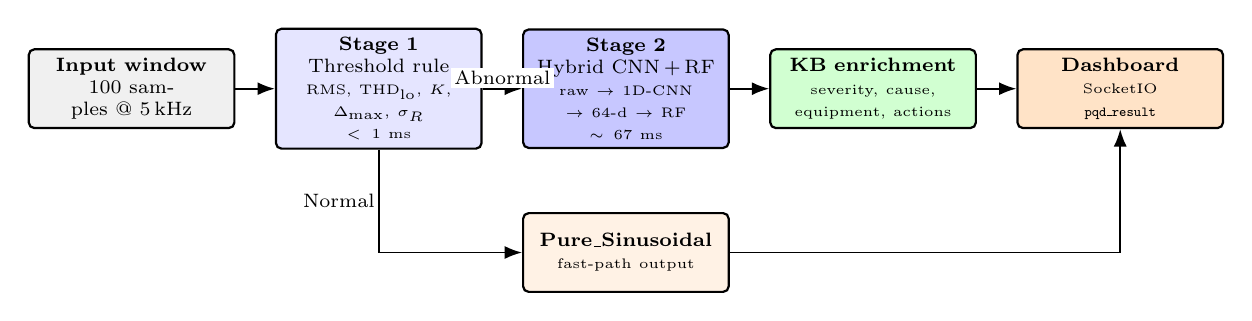
\begin{tikzpicture}[
  font=\scriptsize,
  align=center,
  every path/.style={-{Latex[length=2.2mm]}, thick, line width=0.6pt},
  blk/.style={rectangle, rounded corners=2pt, draw=black, thick,
              minimum height=10mm, text width=2.4cm, inner sep=3pt},
  io/.style={blk, fill=gray!12},
  s1/.style={blk, fill=blue!10},
  s2/.style={blk, fill=blue!22},
  kb/.style={blk, fill=green!18},
  dst/.style={blk, fill=orange!22},
  fast/.style={blk, fill=orange!10, text width=2.4cm},
  lbl/.style={font=\scriptsize, inner sep=1.2pt, fill=white},
]

\node[io]                       (in)   {\textbf{Input window}\\
                                        100 samples @ 5\,kHz};
\node[s1, right=5mm of in]      (st1)  {\textbf{Stage 1}\\Threshold rule\\
                                        {\tiny RMS, THD$_{\mathrm{lo}}$, $K$,}\\
                                        {\tiny $\Delta_{\max}$, $\sigma_R$}\\
                                        {\tiny $<\!1$ ms}};
\node[s2, right=5mm of st1]     (st2)  {\textbf{Stage 2}\\Hybrid CNN\,+\,RF\\
                                        {\tiny raw $\to$ 1D-CNN}\\
                                        {\tiny $\to$ 64-d $\to$ RF}\\
                                        {\tiny $\sim\!67$ ms}};
\node[kb, right=5mm of st2]     (kb)   {\textbf{KB enrichment}\\
                                        {\tiny severity, cause,}\\
                                        {\tiny equipment, actions}};
\node[dst, right=5mm of kb]     (push) {\textbf{Dashboard}\\
                                        {\tiny SocketIO}\\
                                        {\tiny \texttt{pqd\_result}}};

\node[fast, below=8mm of st2]   (norm) {\textbf{Pure\_Sinusoidal}\\
                                        {\tiny fast-path output}};

\draw (in)  -- (st1);
\draw (st1) -- node[lbl, above]{Abnormal} (st2);
\draw (st2) -- (kb);
\draw (kb)  -- (push);

\draw (st1.south) |- node[lbl, near start, left]{Normal} (norm.west);
\draw (norm.east) -| (push.south);

\end{tikzpicture}

  \caption{Two-stage classification architecture. Stage~1 is a
  rule-based threshold detector with a sub-millisecond budget;
  Stage~2 is invoked only on Abnormal windows and is a hybrid
  one-dimensional convolutional neural network feature extractor
  followed by a Random Forest classifier. Each prediction is enriched
  online from an IEEE~1159 knowledge base before being pushed to the
  dashboard.}
  \label{fig:arch}
\end{figure*}

\subsection{Signal Acquisition}
The input to the system is a discrete-time voltage signal
\begin{equation}
  x(n), \quad n = 0, 1, 2, \ldots, N-1,
\end{equation}
where $N = 100$ samples represents one cycle of the 50~Hz fundamental
at $f_s = 5$~kHz. Signals can be sourced from MATLAB, a Python sender,
a JSON HTTP POST request, or a SocketIO event.

\subsection{Preprocessing and Global Normalization}\label{sec:preproc}
In contrast to the conventional per-sample scaling
$\tilde{x}(n) = (x(n) - \mu_x) / \sigma_x$, which removes amplitude
information from each window, the proposed system applies a single
global scale that is computed once on the training set and stored with
the model:
\begin{equation}
  \tilde{x}(n) \;=\; \frac{x(n)}{s}, \qquad
  s \;=\; \mathrm{Q}_{99}\Big(\big\{|x_i^{(\mathrm{train})}|\big\}\Big),
  \label{eq:globalnorm}
\end{equation}
where $\mathrm{Q}_{99}(\cdot)$ denotes the 99th percentile of the
absolute amplitudes of the entire training set. In the present
implementation $s = 2.0535$. The reason per-sample scaling is unsuitable
for amplitude-distinguished PQD classes, and the recovery achieved by
global scaling, are reported in Section~\ref{sec:norm}.

\subsection{Stage 1 --- Threshold Detector}\label{sec:stage1}
Stage~1 computes five features and returns Abnormal if any one of them
exceeds its threshold.

\subsubsection{Root mean square (RMS)}
\begin{equation}
  V_{\mathrm{RMS}} \;=\; \sqrt{\frac{1}{N}\sum_{n=0}^{N-1} x(n)^{2}}.
  \label{eq:rms}
\end{equation}
The detector trips if $V_{\mathrm{RMS}} < 0.65$~pu (sag,
interruption) or $V_{\mathrm{RMS}} > 0.78$~pu (swell).

\subsubsection{Low-order total harmonic distortion approximation}
Using the magnitudes $V_h$ of the $h$-th harmonic bin obtained from
the FFT of the window,
\begin{equation}
  \mathrm{THD}_{\mathrm{lo}} \;=\;
  \frac{\sqrt{V_2^{2} + V_3^{2} + V_5^{2}}}{V_1}.
  \label{eq:thd}
\end{equation}
The detector trips if $\mathrm{THD}_{\mathrm{lo}} > 0.025$ (harmonics,
notch).

\subsubsection{Excess kurtosis}
\begin{equation}
  K \;=\;
  \frac{\frac{1}{N}\sum_{n}\bigl(x(n)-\mu_x\bigr)^{4}}
       {\bigl(\frac{1}{N}\sum_{n}\bigl(x(n)-\mu_x\bigr)^{2}\bigr)^{2}}
   - 3.
  \label{eq:kurt}
\end{equation}
The detector trips if $K > 2.5$ (impulsive transients).

\subsubsection{Maximum consecutive-sample difference}
\begin{equation}
  \Delta_{\max} \;=\;
  \max_{n=1,\ldots,N-1}\;\bigl|x(n) - x(n-1)\bigr|.
  \label{eq:dmax}
\end{equation}
The detector trips if $\Delta_{\max} > 0.15$~pu (notch, oscillatory
burst).

\subsubsection{Quarter-window RMS dispersion}
The window is partitioned into four quarters of length $N/4 = 25$, and
the RMS $r_q$ of each quarter is computed; the dispersion is
\begin{equation}
  \sigma_R \;=\;
  \mathrm{std}\bigl(r_1, r_2, r_3, r_4\bigr).
  \label{eq:qrms}
\end{equation}
The detector trips if $\sigma_R > 0.020$ (flicker).

All five features are $O(N)$ on the 100-sample window, yielding a
Stage~1 budget below 1~ms on a generic CPU. The decision procedure is
summarized in Algorithm~\ref{alg:stage1}.

\begin{algorithm}[t]
\caption{Stage~1 threshold detector}\label{alg:stage1}
\begin{algorithmic}[1]
\Require window $x[0..N-1]$, $N = 100$
\State $V_{\mathrm{RMS}} \gets$ Eq.~\eqref{eq:rms}
\If{$V_{\mathrm{RMS}} \notin [0.65, 0.78]$} \Return Abnormal \EndIf
\State $\mathrm{THD}_{\mathrm{lo}} \gets$ Eq.~\eqref{eq:thd}
\If{$\mathrm{THD}_{\mathrm{lo}} > 0.025$} \Return Abnormal \EndIf
\State $K \gets$ Eq.~\eqref{eq:kurt}
\If{$K > 2.5$} \Return Abnormal \EndIf
\State $\Delta_{\max} \gets$ Eq.~\eqref{eq:dmax}
\If{$\Delta_{\max} > 0.15$} \Return Abnormal \EndIf
\State $\sigma_R \gets$ Eq.~\eqref{eq:qrms}
\If{$\sigma_R > 0.020$} \Return Abnormal \EndIf
\State \Return Normal
\end{algorithmic}
\end{algorithm}

The thresholds are deliberately set on the conservative side. The role
of Stage~1 is not to perform fine-grained classification but to filter
clean traffic out of the heavier inference path while maintaining a
zero Abnormal-as-Normal misclassification rate.

\subsection{Stage 2 --- Hybrid 1D-CNN and Random Forest}
\label{sec:stage2}
Stage~2 produces the seventeen-class decision. The 1D-CNN does not
output class logits at inference time; instead, its penultimate layer
provides a 64-dimensional feature vector that is consumed by a Random
Forest classifier.

\subsubsection{Multi-domain feature foundation (legacy reference)}
For the legacy 36-feature baseline employed in the model-comparison
study (Section~\ref{sec:cmp}), features are extracted across three
domains.

\textit{Time domain (14 features):} including RMS (Eq.~\ref{eq:rms}),
mean
\begin{equation}
  \mu_x \;=\; \frac{1}{N}\sum_{n=0}^{N-1} x(n),
\end{equation}
crest factor
\begin{equation}
  \mathrm{CF} \;=\; \frac{V_{\mathrm{peak}}}{V_{\mathrm{RMS}}},
\end{equation}
peak amplitude, kurtosis, skewness, zero-crossing rate, and
quarter-window statistics.

\textit{Frequency domain (10 features):} including the full total
harmonic distortion
\begin{equation}
  \mathrm{THD} \;=\; \frac{\sqrt{\sum_{h=2}^{H} V_h^{2}}}{V_1},
  \label{eq:thd_full}
\end{equation}
the magnitudes of the first ten harmonic bins of the FFT, and the
fundamental amplitude $V_1$.

\textit{Wavelet domain (12 features):} obtained from a three-level
Daubechies-4 discrete wavelet transform. The energy at decomposition
level $j$ is
\begin{equation}
  E_j \;=\; \sum_{k=1}^{M_j} \bigl|d_{j,k}\bigr|^{2},
  \label{eq:wavelet}
\end{equation}
where $d_{j,k}$ is the $k$-th detail coefficient at level $j$ and
$M_j$ is the number of coefficients at that level.

\subsubsection{1D-CNN feature extractor}
The globally normalized window $\tilde{x}$ (Eq.~\ref{eq:globalnorm})
is supplied directly to a compact 1D-CNN whose architecture is
specified as follows:
\begin{enumerate}
  \item Three convolutional blocks of the form
        $\textrm{Conv1D}(k=5,\,c) \rightarrow \textrm{BatchNorm}
        \rightarrow \textrm{ReLU} \rightarrow \textrm{MaxPool}(2)$,
        with channel widths $c \in \{16, 32, 64\}$.
  \item A global average pooling layer that collapses the temporal
        axis.
  \item A fully connected hidden layer with 128 units and ReLU
        activation.
  \item A 64-unit feature layer; its activation forms the feature
        vector $\mathbf{f} \in \mathbb{R}^{64}$.
  \item A softmax output head used during training only.
\end{enumerate}

The CNN is trained for at most 80 epochs using Adam with an initial
learning rate of $10^{-3}$ and an early-stopping criterion on
validation accuracy with patience 10 and best-weights restoration.
Additive white Gaussian noise at 40~dB SNR is applied online to each
training batch. After training, the softmax head is removed and the
network is retained as a fixed feature extractor.

\subsubsection{Random Forest head}
A Random Forest with $T = 200$ decision trees and
$\mathtt{max\_features} = \log_{2}(d)$ where $d = 64$ is trained on
the CNN feature vectors. At inference, the prediction is the majority
vote
\begin{equation}
  \hat{y} \;=\;
  \mathrm{mode}\bigl(\hat{y}_1, \hat{y}_2, \ldots, \hat{y}_T\bigr),
  \label{eq:vote}
\end{equation}
and the class probability is the empirical frequency of each label
across the trees. This formulation provides a calibrated top-$K$
distribution, which the dashboard uses to display the top three
candidate classes.

\subsubsection{Rationale for the hybrid configuration}
A CNN with a softmax output head converges to comparable accuracy on
this dataset. The hybrid configuration is preferred for two reasons.
First, the Random Forest provides a calibrated top-$K$ probability
distribution without further post-hoc calibration steps such as
temperature scaling or Platt scaling. Second, the modular separation
of the feature extractor and the classifier permits the Random Forest
head to be re-tuned on the frozen feature space within seconds,
without re-training the CNN. This property is operationally
advantageous for field deployments that require periodic drift
adaptation or rapid re-validation.

\subsection{Knowledge-Base Enrichment}\label{sec:kb}
Each Stage~2 prediction $\hat{y}$ is augmented at run time with five
fields drawn from a 17-entry knowledge base derived from
IEEE~Standard~1159: \emph{display name} (human-readable label),
\emph{severity} $\in$ \{none, low, medium, high, critical\},
\emph{cause} (a two-sentence physical explanation),
\emph{equipment-at-risk} (the loads typically affected), and
\emph{immediate actions} (three to five operator-level steps). The
enrichment is a deterministic lookup rather than a model output, but
it transforms the bare class label into actionable diagnostic content.

\subsection{Hyperparameter Optimization}
The Stage~2 Random Forest hyperparameters are optimized using
\texttt{RandomizedSearchCV} with five-fold cross-validation on the
training set. Table~\ref{tab:hp} summarizes the search space and the
selected configuration. Twenty-four combinations were evaluated; the
top thirteen configurations were observed to lie within $\pm 0.05$
percentage points of one another, indicating that the classifier's
accuracy is saturated on the deployed feature space.

\begin{table}[t]
  \centering
  \caption{Hyperparameter optimization for the Stage 2 Random Forest.}
  \label{tab:hp}
  \begin{tabular}{lll}
    \toprule
    Hyperparameter & Search space & Selected value \\
    \midrule
    \texttt{n\_estimators}     & \{100, 200, 500\} & 200 \\
    \texttt{max\_depth}        & \{None, 20, 40, 60\} & None \\
    \texttt{max\_features}     & \{sqrt, log2\} & log2 \\
    \texttt{min\_samples\_split} & \{2, 5, 10\} & 2 \\
    \texttt{min\_samples\_leaf}  & \{1, 2, 4\}  & 1 \\
    \texttt{class\_weight}     & \{None, balanced\} & None \\
    \bottomrule
  \end{tabular}
\end{table}

\subsection{Computational Complexity and Real-Time Considerations}
For an $N$-sample window the computational cost of each stage is as
follows:
\begin{itemize}
  \item \textbf{Stage~1.} Each of the five features is $O(N)$, with the
        FFT-based total harmonic distortion approximation requiring
        $O(N\log N)$ on a fixed-size buffer. The total measured
        latency is below 1~ms for $N = 100$ on a single-thread CPU.
  \item \textbf{Stage~2 CNN forward pass.} 216{,}049 floating-point
        operations per window are required, dominated by the three
        Conv1D layers. The measured mean latency is approximately
        40~ms.
  \item \textbf{Stage~2 Random Forest predict.} The cost is
        $O(T\,d_{\max})$ for $T = 200$ trees on the 64-dimensional
        feature vector. The measured mean latency is approximately
        26~ms.
  \item \textbf{End-to-end Abnormal path.} Approximately 67~ms per
        window, equivalent to approximately three cycles of the 50~Hz
        fundamental.
\end{itemize}

The pipeline is engineered for single-thread CPU inference. The deep
learning framework's graph caches are warmed at backend start-up using
50 dummy windows, ensuring that the first live inference matches
steady-state latency. The dashboard maintains a synthetic-mode
fallback so that user-interface demonstration is independent of
backend reachability. The intended deployment surface is illustrated
in Fig.~\ref{fig:deploy}: voltage and current signals from the grid,
solar inverters, and distributed generation are acquired through a
sensing front-end (e.g., ZMPT101B and ACS712 modules), routed to an
edge compute node (Raspberry~Pi, ESP32, or ARM-class microcontroller)
that executes the trained model, and forwarded over RS485/Modbus or
SocketIO to a panel meter or a SCADA human--machine interface for
operator review.

\begin{figure*}[t]
  \centering
  % Practical deployment-architecture diagram (TikZ).
% Drop-in replacement for figures/deployment.png.
% Used in main.tex as:  % Practical deployment-architecture diagram (TikZ).
% Drop-in replacement for figures/deployment.png.
% Used in main.tex as:  % Practical deployment-architecture diagram (TikZ).
% Drop-in replacement for figures/deployment.png.
% Used in main.tex as:  \input{figures/deployment}
%
% Requires: \usepackage{tikz}
%           \usetikzlibrary{shapes.geometric, arrows.meta, positioning, calc}

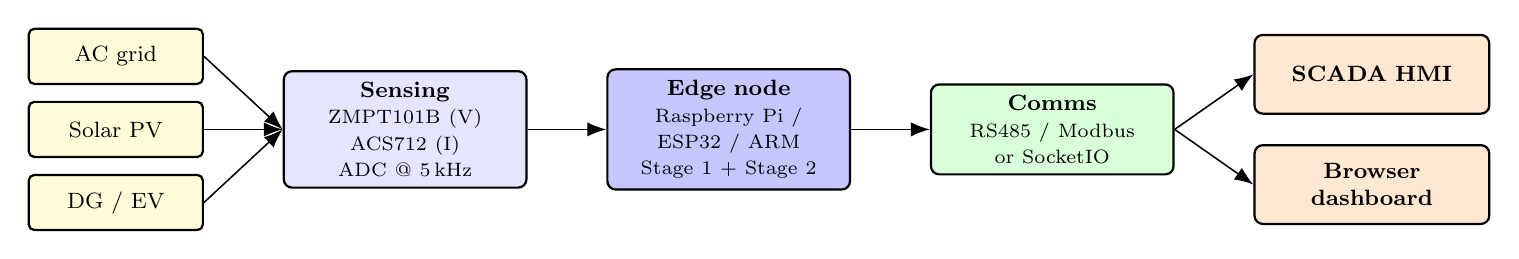
\begin{tikzpicture}[
  font=\footnotesize,
  align=center,
  every path/.style={-{Latex[length=2.4mm]}, thick, line width=0.55pt},
  src/.style={rectangle, rounded corners=2pt, draw=black, thick,
              fill=yellow!15, minimum height=7mm,
              text width=2.0cm, inner sep=3pt},
  proc/.style={rectangle, rounded corners=3pt, draw=black, thick,
               minimum height=10mm, text width=2.8cm, inner sep=4pt},
  bus/.style={proc, fill=green!15},
  hmi/.style={proc, fill=orange!18, text width=2.7cm},
]

% Sources column
\node[src]                          (grid) {AC grid};
\node[src, below=2mm of grid]       (pv)   {Solar PV};
\node[src, below=2mm of pv]         (dg)   {DG / EV};

% Sensing front-end
\node[proc, fill=blue!10, right=10mm of pv] (sense)
  {\textbf{Sensing}\\
   {\scriptsize ZMPT101B (V)}\\
   {\scriptsize ACS712 (I)}\\
   {\scriptsize ADC @ 5\,kHz}};

% Edge compute (running this paper's pipeline)
\node[proc, fill=blue!22, right=10mm of sense] (edge)
  {\textbf{Edge node}\\
   {\scriptsize Raspberry Pi /}\\
   {\scriptsize ESP32 / ARM}\\
   {\scriptsize Stage~1 + Stage~2}};

% Communication bus
\node[bus, right=10mm of edge] (bus)
  {\textbf{Comms}\\
   {\scriptsize RS485 / Modbus}\\
   {\scriptsize or SocketIO}};

% Outputs (HMIs)
\node[hmi, right=10mm of bus, yshift=7mm]  (scada) {\textbf{SCADA HMI}};
\node[hmi, right=10mm of bus, yshift=-7mm] (dash)  {\textbf{Browser dashboard}};

% Edges
\draw (grid.east) -- (sense.west);
\draw (pv.east)   -- (sense.west);
\draw (dg.east)   -- (sense.west);
\draw (sense)     -- (edge);
\draw (edge)      -- (bus);
\draw (bus.east)  -- (scada.west);
\draw (bus.east)  -- (dash.west);

\end{tikzpicture}

%
% Requires: \usepackage{tikz}
%           \usetikzlibrary{shapes.geometric, arrows.meta, positioning, calc}

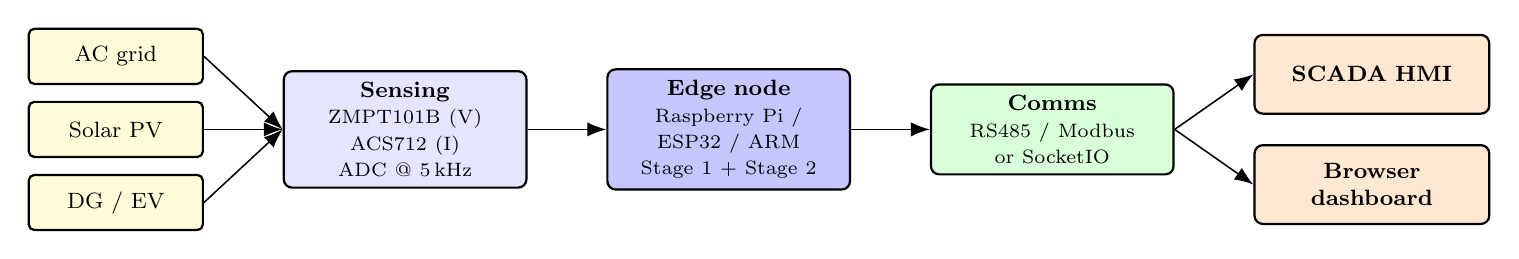
\begin{tikzpicture}[
  font=\footnotesize,
  align=center,
  every path/.style={-{Latex[length=2.4mm]}, thick, line width=0.55pt},
  src/.style={rectangle, rounded corners=2pt, draw=black, thick,
              fill=yellow!15, minimum height=7mm,
              text width=2.0cm, inner sep=3pt},
  proc/.style={rectangle, rounded corners=3pt, draw=black, thick,
               minimum height=10mm, text width=2.8cm, inner sep=4pt},
  bus/.style={proc, fill=green!15},
  hmi/.style={proc, fill=orange!18, text width=2.7cm},
]

% Sources column
\node[src]                          (grid) {AC grid};
\node[src, below=2mm of grid]       (pv)   {Solar PV};
\node[src, below=2mm of pv]         (dg)   {DG / EV};

% Sensing front-end
\node[proc, fill=blue!10, right=10mm of pv] (sense)
  {\textbf{Sensing}\\
   {\scriptsize ZMPT101B (V)}\\
   {\scriptsize ACS712 (I)}\\
   {\scriptsize ADC @ 5\,kHz}};

% Edge compute (running this paper's pipeline)
\node[proc, fill=blue!22, right=10mm of sense] (edge)
  {\textbf{Edge node}\\
   {\scriptsize Raspberry Pi /}\\
   {\scriptsize ESP32 / ARM}\\
   {\scriptsize Stage~1 + Stage~2}};

% Communication bus
\node[bus, right=10mm of edge] (bus)
  {\textbf{Comms}\\
   {\scriptsize RS485 / Modbus}\\
   {\scriptsize or SocketIO}};

% Outputs (HMIs)
\node[hmi, right=10mm of bus, yshift=7mm]  (scada) {\textbf{SCADA HMI}};
\node[hmi, right=10mm of bus, yshift=-7mm] (dash)  {\textbf{Browser dashboard}};

% Edges
\draw (grid.east) -- (sense.west);
\draw (pv.east)   -- (sense.west);
\draw (dg.east)   -- (sense.west);
\draw (sense)     -- (edge);
\draw (edge)      -- (bus);
\draw (bus.east)  -- (scada.west);
\draw (bus.east)  -- (dash.west);

\end{tikzpicture}

%
% Requires: \usepackage{tikz}
%           \usetikzlibrary{shapes.geometric, arrows.meta, positioning, calc}

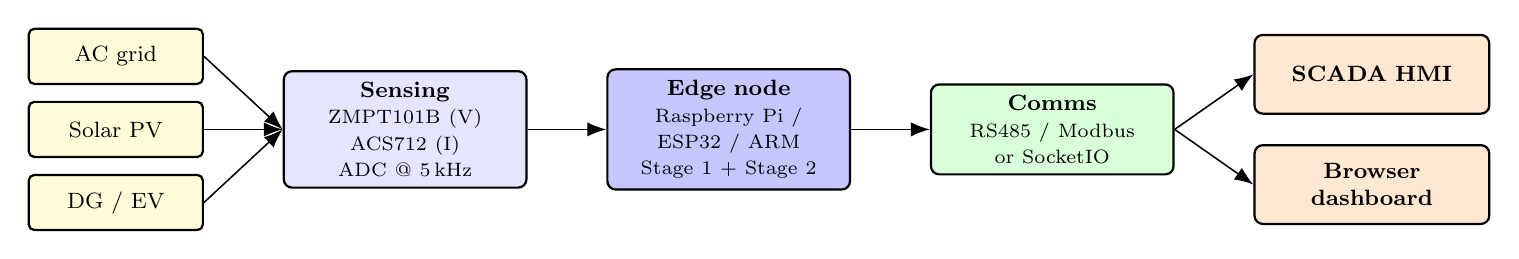
\begin{tikzpicture}[
  font=\footnotesize,
  align=center,
  every path/.style={-{Latex[length=2.4mm]}, thick, line width=0.55pt},
  src/.style={rectangle, rounded corners=2pt, draw=black, thick,
              fill=yellow!15, minimum height=7mm,
              text width=2.0cm, inner sep=3pt},
  proc/.style={rectangle, rounded corners=3pt, draw=black, thick,
               minimum height=10mm, text width=2.8cm, inner sep=4pt},
  bus/.style={proc, fill=green!15},
  hmi/.style={proc, fill=orange!18, text width=2.7cm},
]

% Sources column
\node[src]                          (grid) {AC grid};
\node[src, below=2mm of grid]       (pv)   {Solar PV};
\node[src, below=2mm of pv]         (dg)   {DG / EV};

% Sensing front-end
\node[proc, fill=blue!10, right=10mm of pv] (sense)
  {\textbf{Sensing}\\
   {\scriptsize ZMPT101B (V)}\\
   {\scriptsize ACS712 (I)}\\
   {\scriptsize ADC @ 5\,kHz}};

% Edge compute (running this paper's pipeline)
\node[proc, fill=blue!22, right=10mm of sense] (edge)
  {\textbf{Edge node}\\
   {\scriptsize Raspberry Pi /}\\
   {\scriptsize ESP32 / ARM}\\
   {\scriptsize Stage~1 + Stage~2}};

% Communication bus
\node[bus, right=10mm of edge] (bus)
  {\textbf{Comms}\\
   {\scriptsize RS485 / Modbus}\\
   {\scriptsize or SocketIO}};

% Outputs (HMIs)
\node[hmi, right=10mm of bus, yshift=7mm]  (scada) {\textbf{SCADA HMI}};
\node[hmi, right=10mm of bus, yshift=-7mm] (dash)  {\textbf{Browser dashboard}};

% Edges
\draw (grid.east) -- (sense.west);
\draw (pv.east)   -- (sense.west);
\draw (dg.east)   -- (sense.west);
\draw (sense)     -- (edge);
\draw (edge)      -- (bus);
\draw (bus.east)  -- (scada.west);
\draw (bus.east)  -- (dash.west);

\end{tikzpicture}

  \caption{Practical deployment architecture. Multi-source signal
  acquisition is followed by a sensing front-end, edge-compute
  inference using the proposed pipeline, and an RS485 or SocketIO
  link to the monitoring human--machine interface.}
  \label{fig:deploy}
\end{figure*}

% =====================================================================
\section{Real-Time Backend and Dashboard}\label{sec:realtime}
% =====================================================================
The classifier is encapsulated within a Flask and Flask-SocketIO
server. Three input paths are exposed: a JSON \texttt{POST /api/predict}
endpoint for one-shot HTTP queries, a SocketIO \texttt{predict} event
for low-latency clients, and a TCP listener on port 5555 that accepts
newline-delimited JSON frames of the form
\texttt{\{label, signal:[v0..v99], window\}}. The TCP listener
broadcasts each prediction as a SocketIO \texttt{pqd\_result} event to
all connected dashboards. Both the included MATLAB sender and the
Python sender, the latter implementing realistic synthetic IEEE~1159
signal generation, employ this path.

\begin{figure}[t]
  \centering
  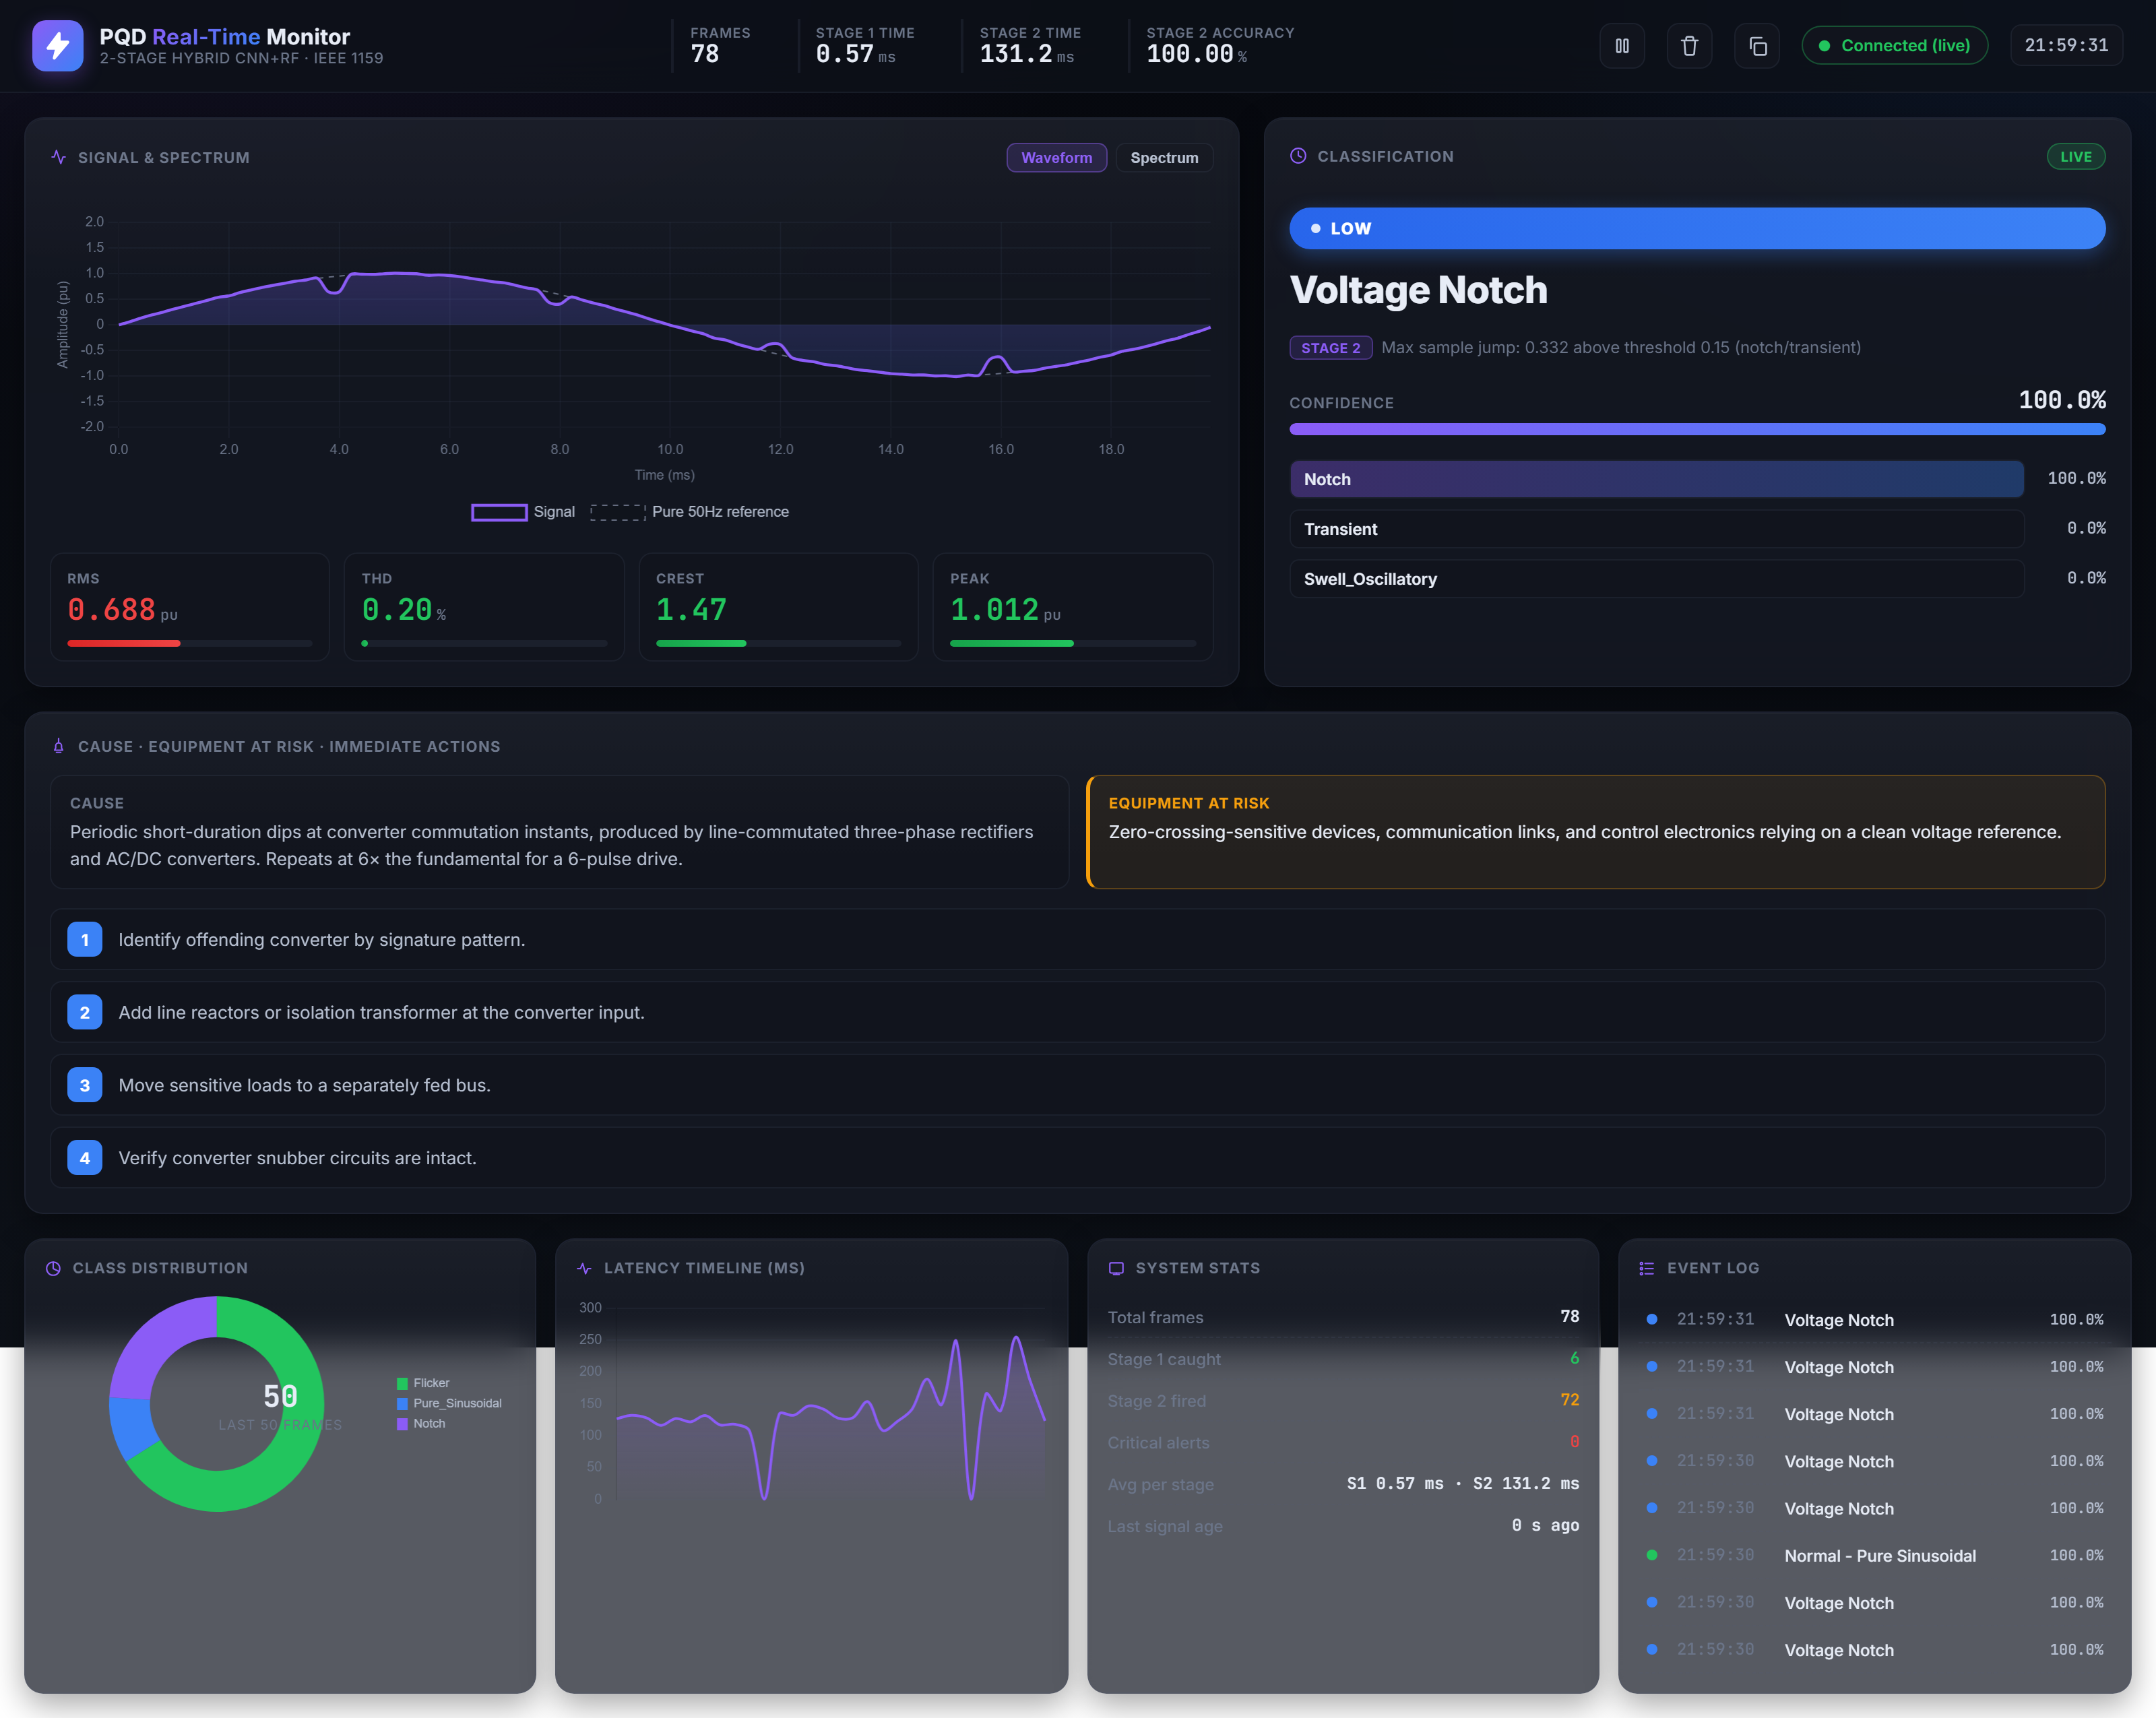
\includegraphics[width=0.95\columnwidth]{figures/dashboard.png}
  \caption{Live dashboard. Six panels are rendered: waveform and
  spectrum, signal parameters, the classification card with top-three
  candidates, cause and equipment-at-risk, recommended operator
  actions, and a system-statistics strip with a rolling latency
  timeline. The dashboard automatically falls back to a built-in
  demonstration mode if the backend is unreachable for three seconds.}
  \label{fig:dashboard}
\end{figure}

The dashboard, illustrated in Fig.~\ref{fig:dashboard}, is implemented
as a single-file HTML/CSS/JavaScript page using Chart.js and
Socket.IO. Six panels are rendered: the live waveform with a tabbed
FFT spectrum view, a gauge cluster for RMS, total harmonic distortion,
crest factor, and peak amplitude, a classification card displaying a
severity badge and top-three confidence bars, a card containing the
cause and equipment-at-risk fields, a list of the recommended
operator actions, and a system-statistics strip showing the number of
frames received, both stage latencies, and a rolling latency timeline.

% =====================================================================
\section{Experimental Setup}\label{sec:exp}
% =====================================================================
\subsection{Hardware}
All measurements are conducted on a single laptop-class workstation:
Windows on AMD64 with an Intel 8-thread CPU. Single-thread evaluation
is enforced. No GPU is used, and no cloud service is contacted at
inference time.

\subsection{Test Workload}
Inference latency is measured on the full 3{,}400-sample test set,
with one sample per call. A 50-iteration warm-up is applied to all
neural-network models to eliminate graph-caching effects from the
timed window. The Random Forest classifier is warmed by a single
forward pass.

\subsection{Performance Metrics}
Reported metrics include overall accuracy, per-class precision,
recall, F1 score, the confusion matrix, latency at the 50th and 95th
percentiles and at the mean, parameter count, and on-disk model size.
End-to-end pipeline accuracy is reported on a 510-signal balanced
mixed-traffic test composed of 30\% Normal and 70\% Abnormal traffic.

% =====================================================================
\section{Model Comparison and Selection}\label{sec:cmp}
% =====================================================================
Prior to adoption of the hybrid CNN-RF design, six classical machine
learning algorithms were trained on the same 36-feature multi-domain
vector under identical conditions. The algorithms considered were
Logistic Regression, Support Vector Machine (SVM), $k$-Nearest
Neighbours ($k$NN), Decision Tree, Gradient Boosting, and Random
Forest. Performance on the XPQRS dataset and on a second PQ dataset
(the PQ Disturbances Dataset, with pre-extracted features) is
reported in Table~\ref{tab:modelcmp}.

\begin{table}[t]
  \centering
  \caption{Comparison of classical machine learning models on two
           datasets. Accuracy and macro F1 are reported on the
           held-out test split.}
  \label{tab:modelcmp}
  \begin{tabular}{lcccc}
    \toprule
    Model & XPQRS Acc. & PQ Acc. & XPQRS F1 & PQ F1 \\
    \midrule
    Gradient Boosting   & 0.9112 & 0.9837 & 0.9107 & 0.9836 \\
    Random Forest       & 0.9062 & 0.9812 & 0.9056 & 0.9816 \\
    Decision Tree       & 0.8650 & 0.9625 & 0.8646 & 0.9620 \\
    Logistic Regression & 0.8524 & 0.9375 & 0.8489 & 0.9372 \\
    SVM                 & 0.8335 & 0.8812 & 0.8298 & 0.8798 \\
    $k$NN               & 0.8006 & 0.9062 & 0.7955 & 0.9046 \\
    \bottomrule
  \end{tabular}
\end{table}

The Random Forest classifier provides the most favourable combination
of accuracy, robustness, and deployment simplicity within this
comparison and is therefore adopted as the basis for both the legacy
36-feature baseline and the Stage~2 head of the hybrid model. When
combined with the learned 64-dimensional CNN feature representation in
place of the 36 hand-engineered features, the Random Forest head
attains 98.85\% accuracy on the XPQRS test set, an absolute
improvement of 8.23 percentage points over the legacy configuration.
This improvement is attributed to the richer learned feature space.

% =====================================================================
\section{Results and Discussion}\label{sec:results}
% =====================================================================
\subsection{Stage~2 Classification Performance}\label{sec:headline}
The hybrid 1D-CNN and Random Forest classifier achieves an overall
test accuracy of 98.85\% on the held-out 3{,}400-sample test set. The
test set is exactly balanced; macro-averaged precision, recall, and
F1 are therefore equal at 98.85\%. Thirteen of the seventeen classes
attain 100\% recall. The four non-perfect classes are Sag (90.50\%),
Sag-Flicker (91.00\%), Swell (99.50\%), and Swell-Flicker (99.50\%).
The complete per-class breakdown is reported in
Table~\ref{tab:perclass}.

\begin{table}[t]
  \centering
  \caption{Per-class classification performance on the 3,400-sample
           test set, with 200 samples per class.}
  \label{tab:perclass}
  \begin{tabular}{lrrr}
    \toprule
    Class & Recall & Precision & F1 \\
    \midrule
    Pure\_Sinusoidal       & 100.00 & 100.00 & 100.00 \\
    Flicker                & 100.00 & 100.00 & 100.00 \\
    Harmonics              & 100.00 & 100.00 & 100.00 \\
    Harmonics\_Flicker     & 100.00 & 100.00 & 100.00 \\
    Harmonics\_Notch       & 100.00 & 100.00 & 100.00 \\
    Interruption           & 100.00 & 100.00 & 100.00 \\
    Notch                  & 100.00 & 100.00 & 100.00 \\
    Oscillatory\_Transient & 100.00 & 100.00 & 100.00 \\
    Sag\_Harmonics         & 100.00 & 100.00 & 100.00 \\
    Sag\_Oscillatory       & 100.00 & 100.00 & 100.00 \\
    Swell\_Harmonics       & 100.00 & 100.00 & 100.00 \\
    Swell\_Oscillatory     & 100.00 & 100.00 & 100.00 \\
    Transient              & 100.00 & 100.00 & 100.00 \\
    Swell                  & 99.50  & 99.50  & 99.50  \\
    Swell\_Flicker         & 99.50  & 99.50  & 99.50  \\
    Sag\_Flicker           & 91.00  & 90.55  & 90.77  \\
    Sag                    & 90.50  & 90.95  & 90.73  \\
    \midrule
    \textbf{Macro avg}     & \textbf{98.85} & \textbf{98.85}
                           & \textbf{98.85} \\
    \bottomrule
  \end{tabular}
\end{table}

\subsection{Confusion Patterns}
The misclassification errors are not uniformly distributed across the
off-diagonal of the confusion matrix shown in Fig.~\ref{fig:cm}. The
errors concentrate in a single $2 \times 2$ block: nineteen Sag
windows are predicted as Sag\_Flicker, and eighteen Sag\_Flicker
windows are predicted as Sag. Every other off-diagonal entry contains
at most one misclassification. The discriminating feature between Sag
and Sag-with-Flicker is the presence of envelope drift across the
cycle. With $N = 100$ samples at 50~Hz, only one full cycle is
available, and a slow flicker modulation may not have produced an
observable envelope variation within that cycle. A multi-cycle
context window for these classes is identified as a natural
extension and is reserved for future work.

\begin{figure}[t]
  \centering
  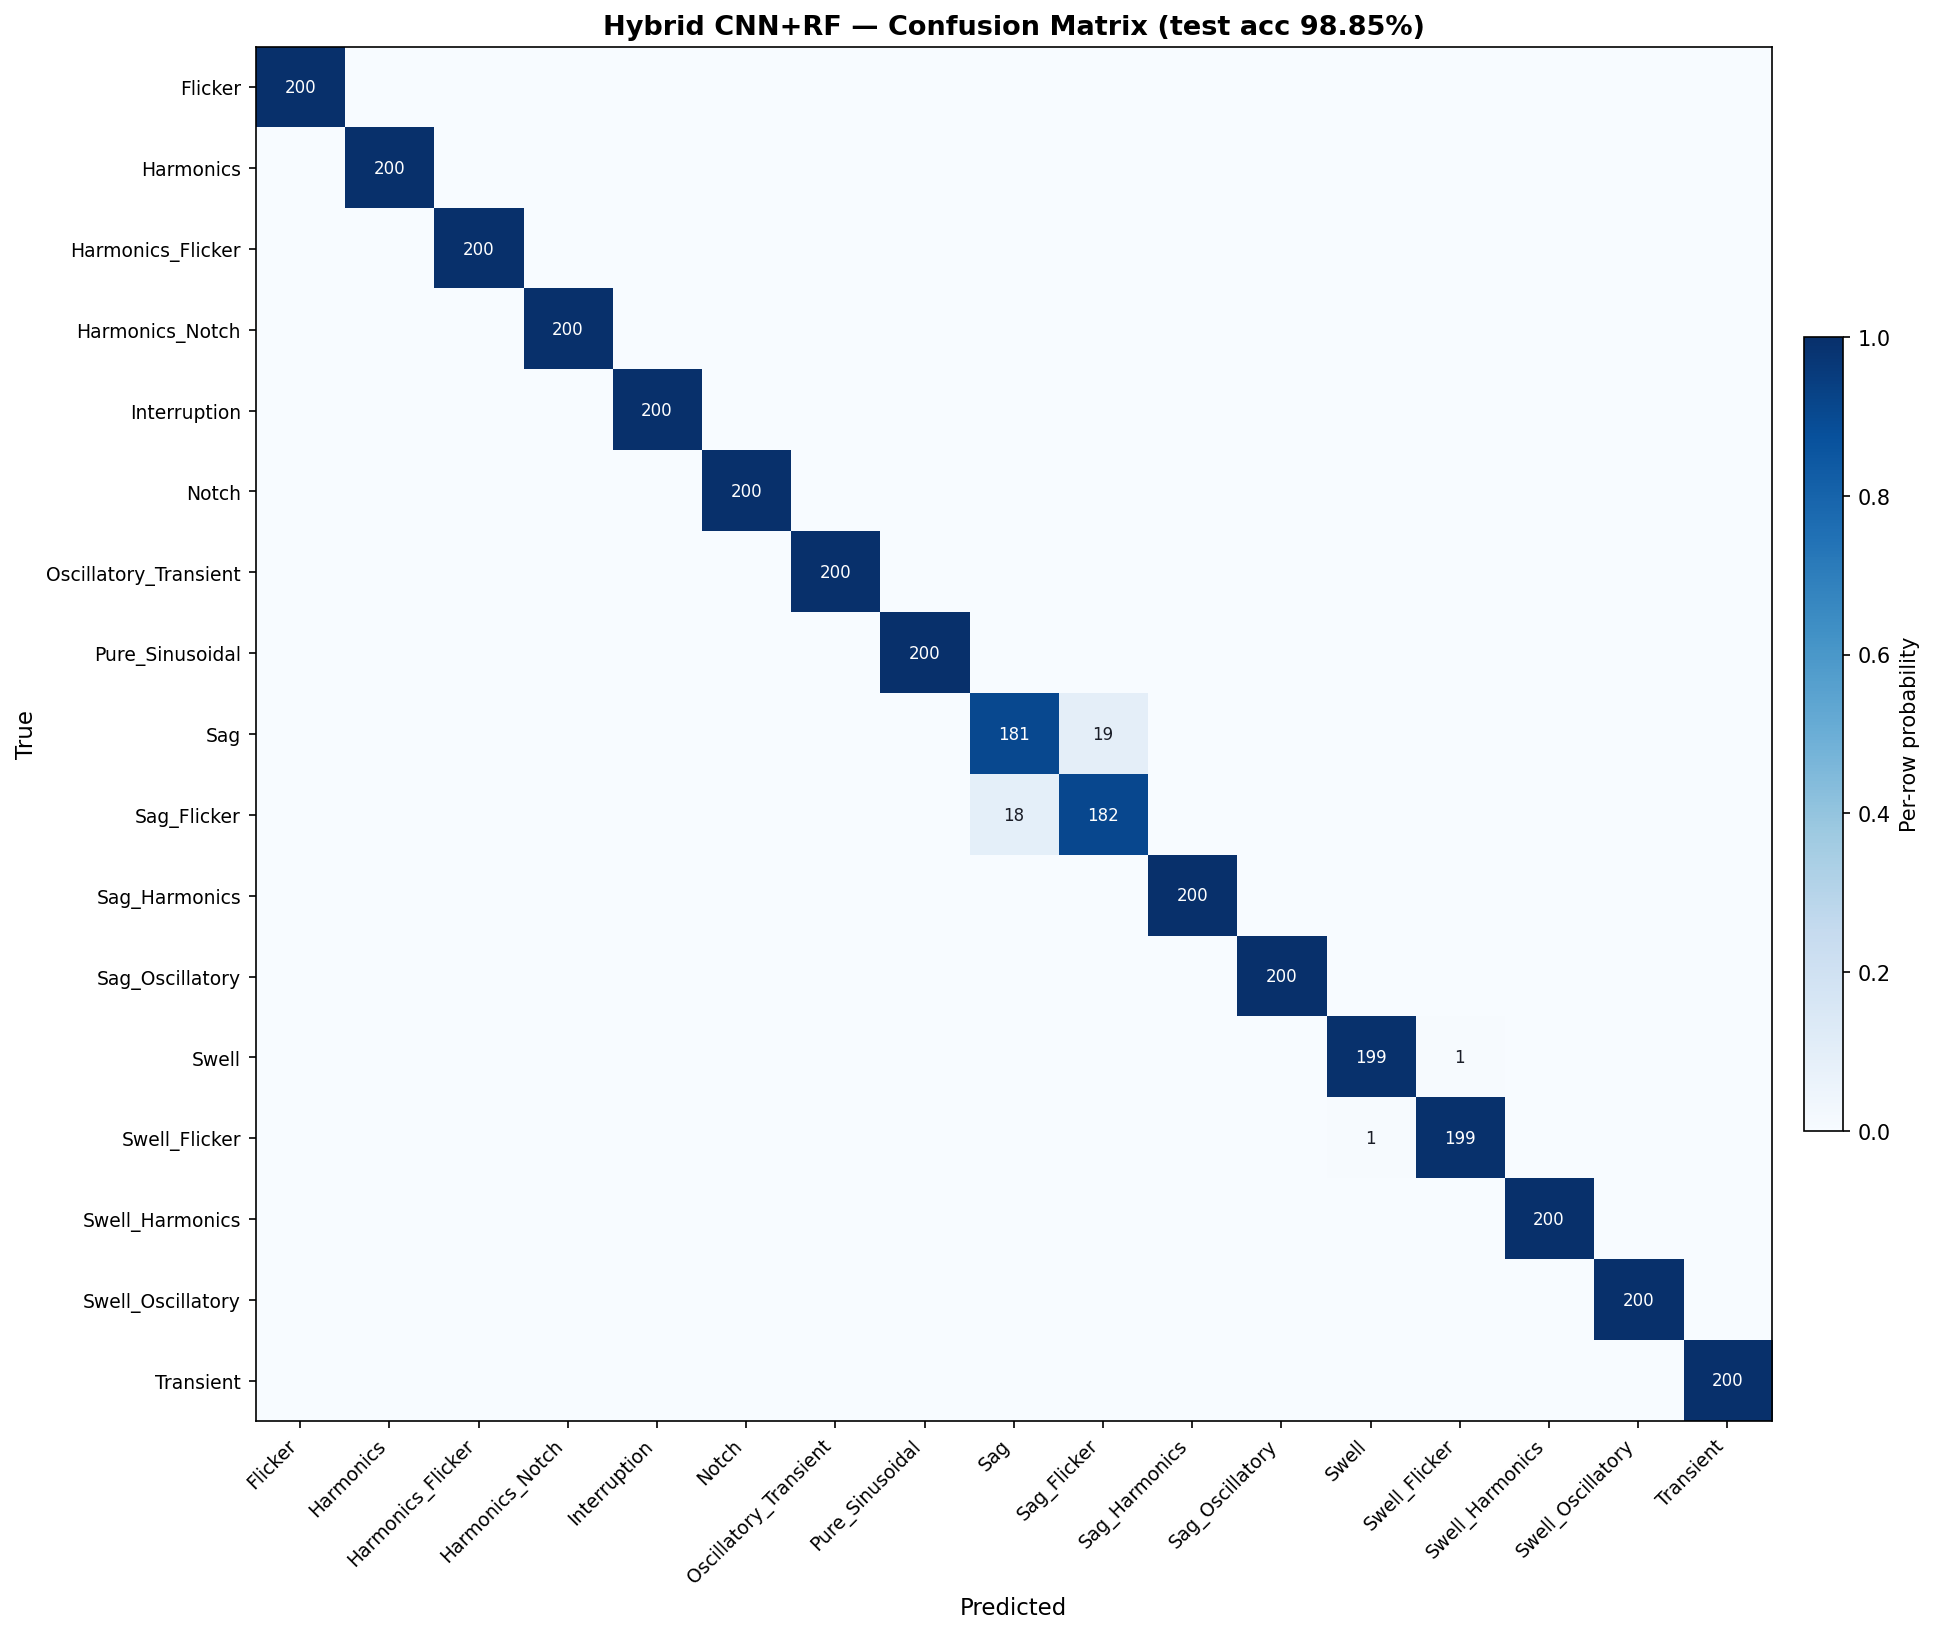
\includegraphics[width=0.98\columnwidth]{figures/confusion_matrix_hybrid.png}
  \caption{Confusion matrix of the hybrid 1D-CNN and Random Forest
  classifier on the 3,400-sample test set. Thirteen of seventeen
  classes attain 100\% recall, and the residual errors are confined
  to a single $2 \times 2$ block between Sag and Sag\_Flicker.}
  \label{fig:cm}
\end{figure}

\subsection{Input-Normalization Analysis}\label{sec:norm}
An initial implementation employed per-sample maximum-absolute
normalization, in which each window is divided by its own peak
amplitude before being supplied to the CNN. This scheme is the
canonical preprocessing step in much of the published deep-learning
PQ literature. Under per-sample normalization, the hybrid model's
test accuracy was observed to be 52.0\%, substantially below the
legacy 36-feature Random Forest baseline.

The mechanism underlying this collapse is straightforward. After
per-sample maximum-absolute normalization, a 0.5~pu sag and a 1.0~pu
pure sinusoid both reduce to unit-amplitude sine waves of identical
shape; voltage swells and interruptions are subject to the same
collapse. The amplitude information that distinguishes these classes
is therefore eliminated by the normalizer.

The remedy is to apply a single global scale, computed once on the
training set and stored with the model, in accordance with
Eq.~\eqref{eq:globalnorm}. Under this scheme, the test accuracy
recovered from 52.0\% to 98.85\%, an absolute improvement of 47
percentage points obtained from a single preprocessing modification.
This finding is transferable to any deep-learning PQ pipeline that
includes amplitude-distinguished classes.

\subsection{End-to-End Pipeline Performance}
On the 510-signal mixed-traffic test (30\% Normal, 70\% Abnormal,
balanced across the sixteen Abnormal classes), the end-to-end
pipeline attains an accuracy of 96.67\%. Stage~1 detects 100\% of
Normal windows correctly and produces zero false alarms; no Abnormal
window is misclassified as Normal. The accuracy gap between the
Stage~2 result on its own test set (98.85\%) and the end-to-end
pipeline (96.67\%) is therefore attributable to the Stage~2
misclassifications on Sag and Sag-Flicker, evaluated over a smaller
and less favourable mix.

\subsection{Latency Budget for Edge Deployment}\label{sec:cnnvsrf}
A practical PQ monitor must deliver a decision before the next
decision-relevant window arrives. Stage~1 of the proposed pipeline
satisfies a sub-cycle deadline for 100\% of Normal traffic, completing
in less than one millisecond per window. Stage~2 requires
approximately 67~ms per Abnormal window, equivalent to approximately
three cycles of the 50~Hz fundamental, and is invoked only on windows
that have already been screened as anomalous, ensuring that the heavy
inference path is never exercised on clean traffic.
Table~\ref{tab:latency} reports the per-stage latency budget on a
single-thread laptop CPU.

\begin{table}[t]
  \centering
  \caption{Per-stage latency budget on a single-thread laptop CPU.
           Measurements are steady-state, post warm-up, without GPU
           acceleration or cloud connectivity.}
  \label{tab:latency}
  \begin{tabular}{lrrr}
    \toprule
    Stage & p50 (ms) & Mean (ms) & p95 (ms) \\
    \midrule
    Stage~1 (5 features + decision)        & 0.4  & 0.4  & 0.7  \\
    Stage~2 -- CNN forward pass            & 38   & 40   & 55   \\
    Stage~2 -- Random Forest predict       & 24   & 26   & 38   \\
    Stage~2 -- total (Abnormal path)       & 65   & 67   & 88   \\
    \midrule
    \textbf{End-to-end -- Normal path}     & \textbf{0.4} & \textbf{0.4} & \textbf{0.7} \\
    \textbf{End-to-end -- Abnormal path}   & \textbf{65}  & \textbf{67}  & \textbf{88}  \\
    \bottomrule
  \end{tabular}
\end{table}

A growing portion of the deep-learning PQ literature relies on cloud
inference in order to accommodate model size~\cite{xiao2023iot}. Cloud
deployment, however, introduces a network round-trip-time overhead
before any inference is initiated. Wide-area round-trip times from a
distribution feeder to a regional data centre are typically 100--300~ms
even on a clean wired link, and substantially higher on congested or
wireless paths --- already several multiples of one PQ cycle. The
proposed pipeline performs detection in less than one millisecond and
classification within approximately three cycles, entirely on a single
CPU thread, without GPU acceleration or external service connectivity.
The proposed system therefore satisfies an operational deadline that
cloud-deployed deep PQ classifiers cannot satisfy under realistic
network conditions, while remaining a deeply learned classifier in
Stage~2.

\subsection{Hyperparameter Sensitivity}\label{sec:tuning}
A 24-combination, five-fold cross-validation grid search was conducted
over the Stage~2 Random Forest on the frozen CNN feature space. The
top thirteen configurations clustered within $\pm 0.05$ percentage
points of one another. The deployed configuration (200 trees,
$\log_2$ feature selection) lies inside this cluster. The result
indicates that classification accuracy is saturated on the deployed
feature space, and that further hyperparameter tuning of the Random
Forest head is unlikely to yield improvements that exceed the
statistical noise of the test split.

\subsection{Sample Prediction Outputs}
A representative dashboard output for an Abnormal input is shown in
Fig.~\ref{fig:pred_abn}. The classifier identifies the waveform as
Harmonics with confidence 1.00 and renders the cause and recommended
actions retrieved from the knowledge base. The corresponding output
for a Normal input is shown in Fig.~\ref{fig:pred_norm}: Stage~1
classifies the clean sinusoid as Pure\_Sinusoidal in less than one
millisecond, and Stage~2 is not invoked.

\begin{figure}[t]
  \centering
  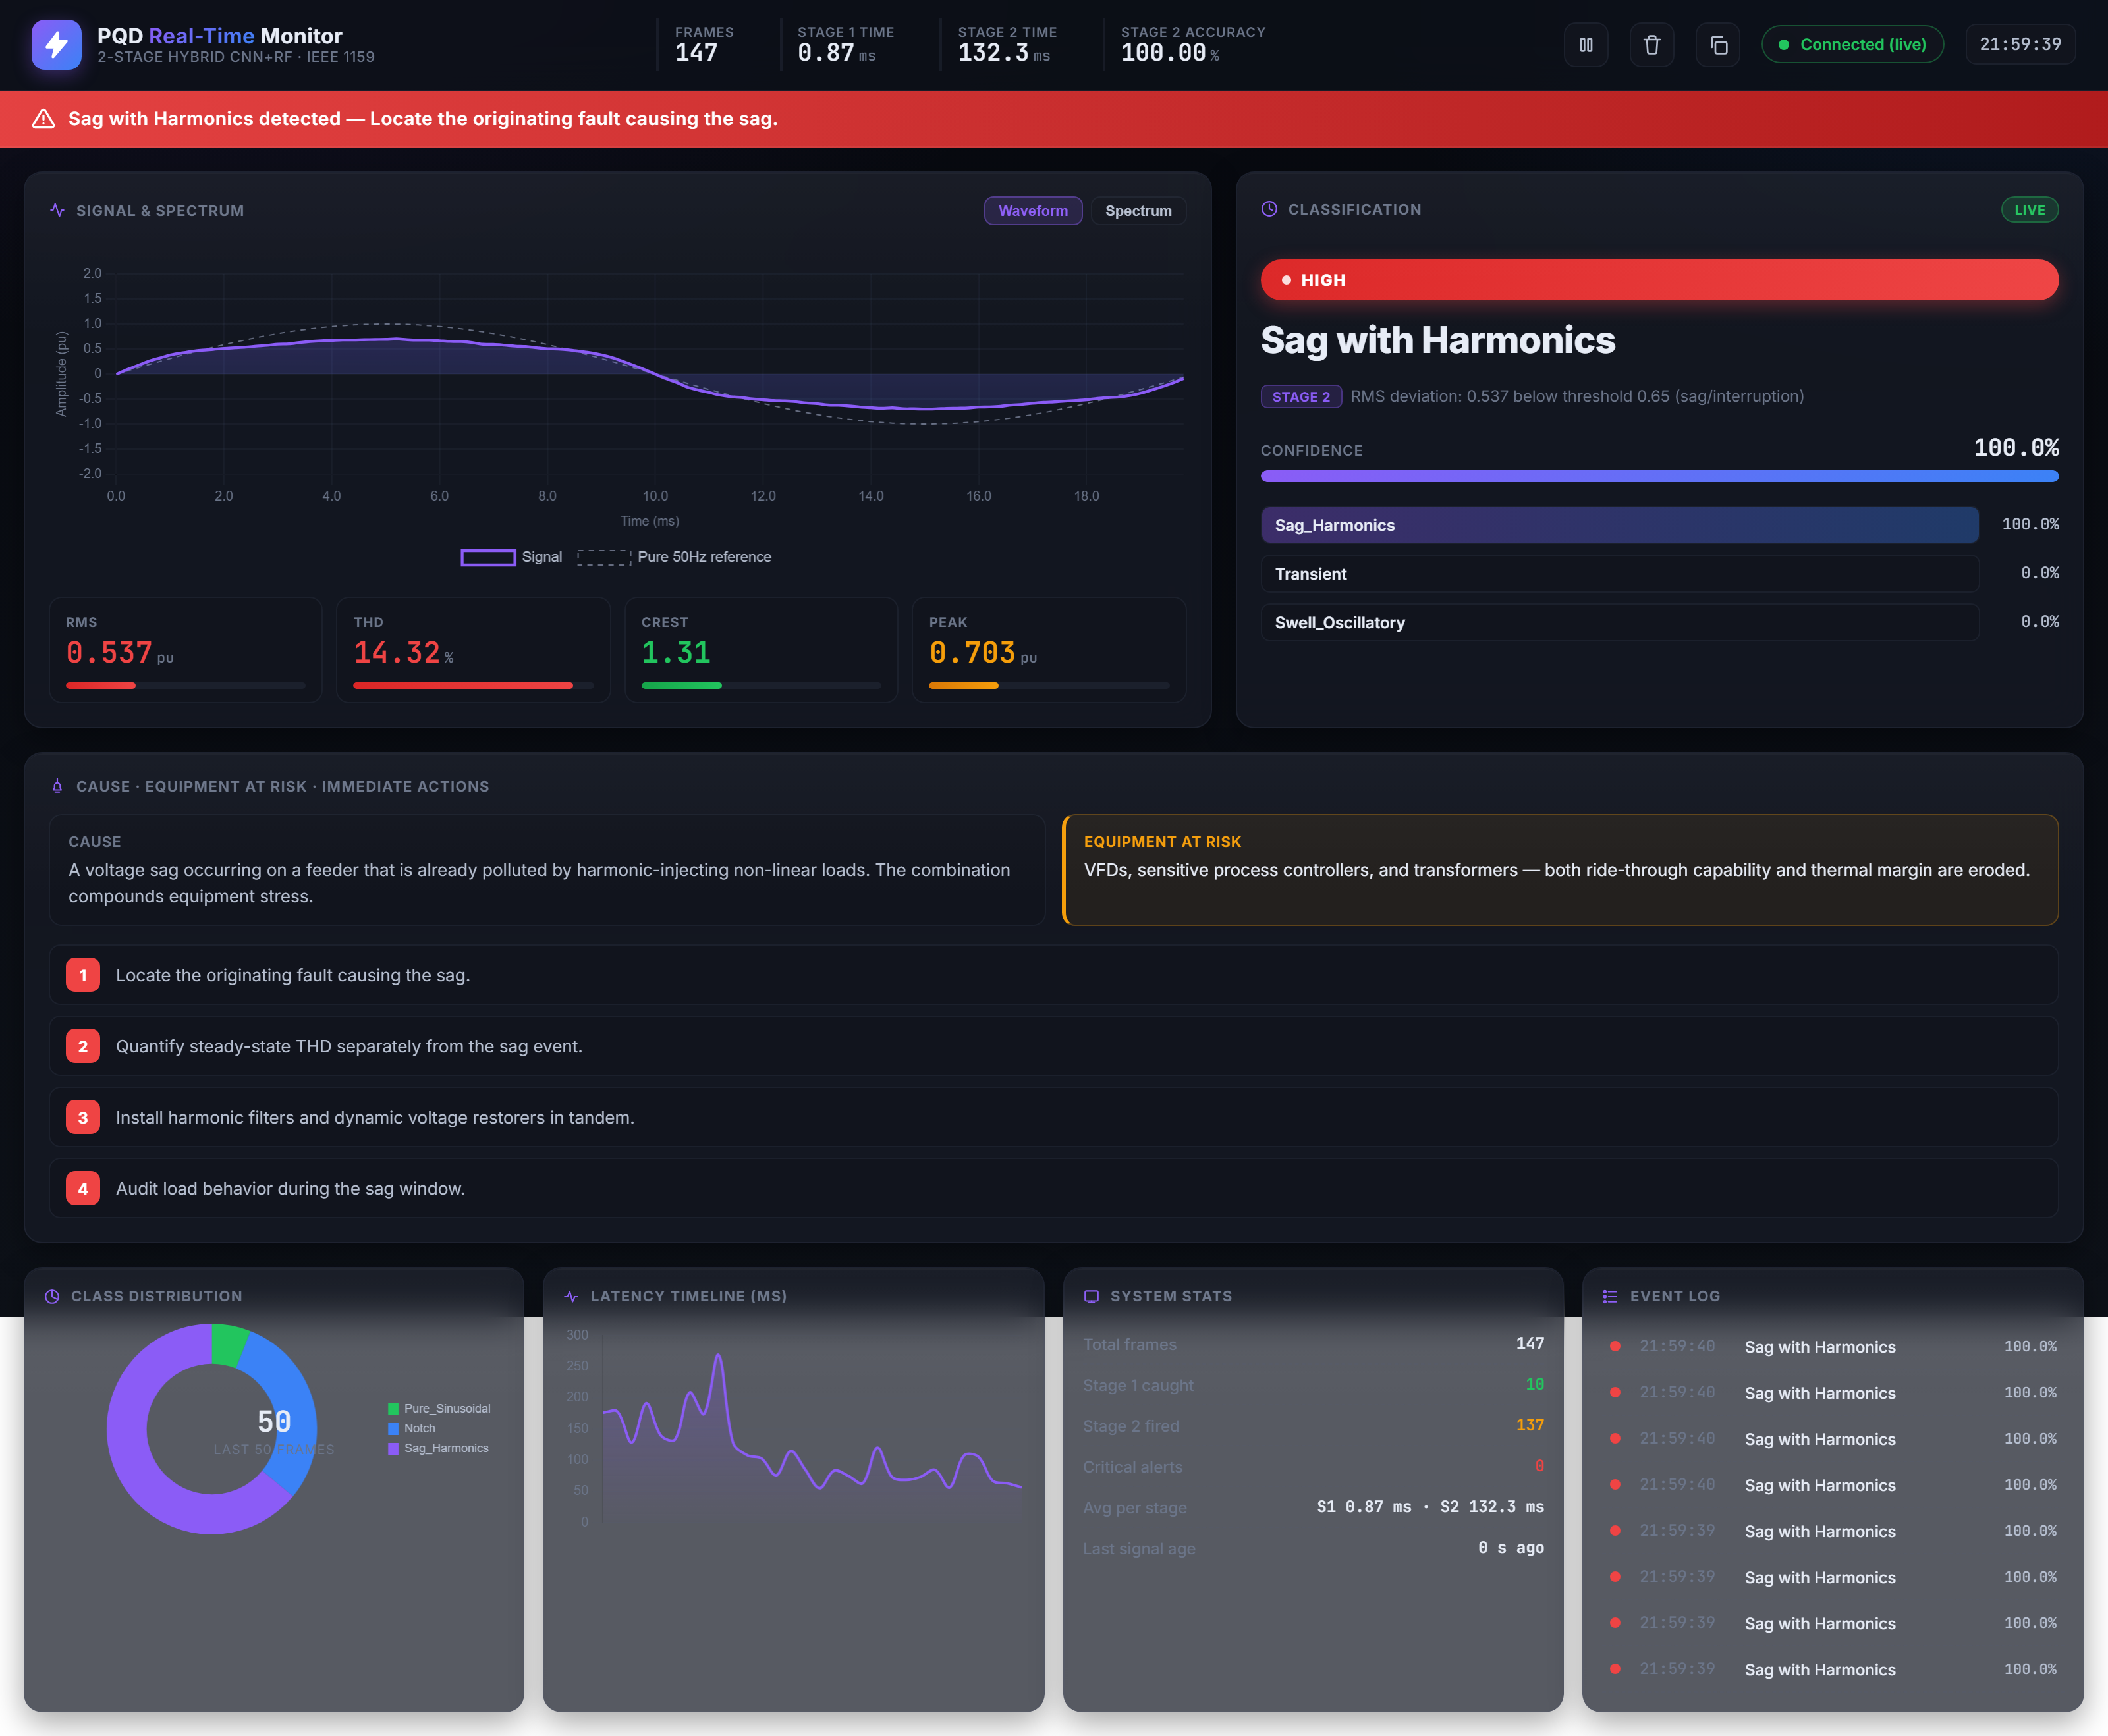
\includegraphics[width=0.95\columnwidth]{figures/pred_abnormal.png}
  \caption{Sample prediction output for an Abnormal input. The
  dashboard shows the waveform on the left, the classification card
  with the predicted class and confidence on the right, and the cause
  and actions card below.}
  \label{fig:pred_abn}
\end{figure}

\begin{figure}[t]
  \centering
  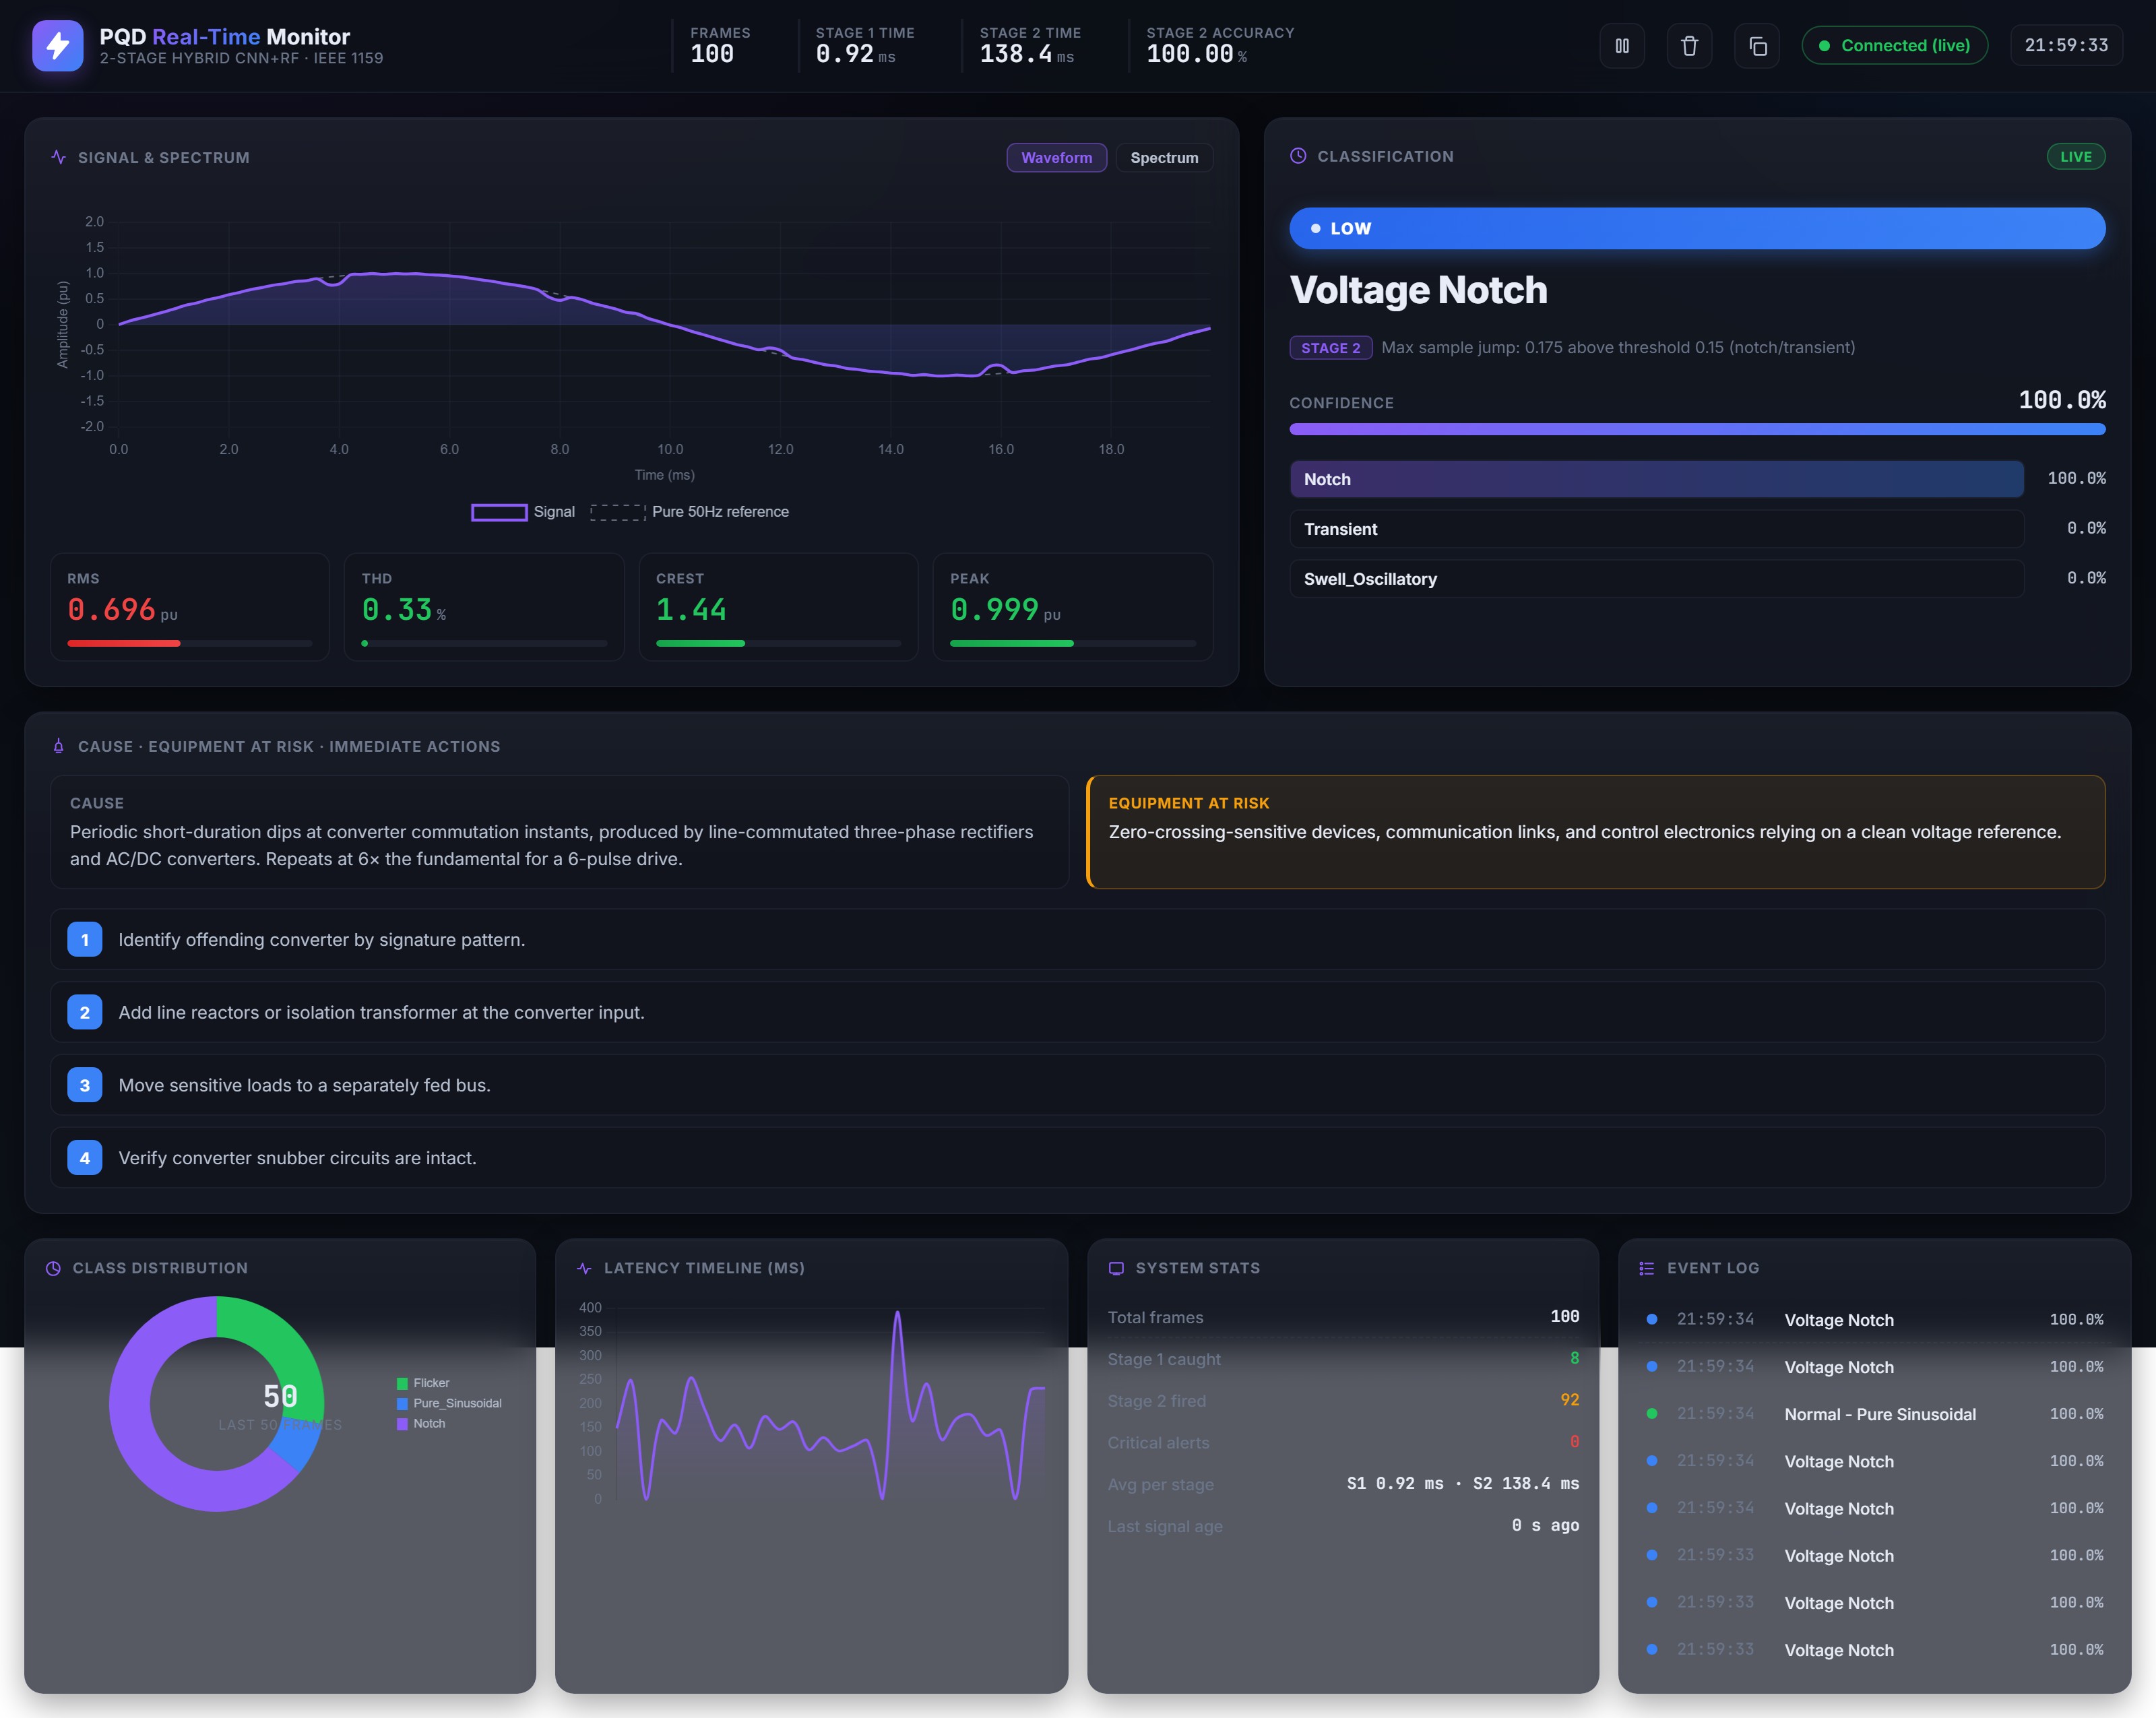
\includegraphics[width=0.95\columnwidth]{figures/pred_normal.png}
  \caption{Sample prediction output for a Normal input. A clean sine
  cycle is classified as Pure\_Sinusoidal by Stage~1 in less than one
  millisecond; Stage~2 is not invoked.}
  \label{fig:pred_norm}
\end{figure}

\subsection{Per-Prediction Interpretability via SHAP}
A TreeSHAP~\cite{lundberg2020trees} explainer is integrated as a
post-hoc attribution layer on the legacy 36-feature Random Forest
baseline. For any single window, the system returns the top three
contributing features along with their physical units (RMS in pu,
total harmonic distortion in percent, harmonic magnitudes, and
wavelet energies) together with the SHAP magnitude and sign of each
contribution. A representative explanation for a Sag prediction
identifies RMS as the dominant feature with a negative SHAP value,
together with two amplitude-correlated wavelet energies. Operators
are therefore able to review borderline classifications using named
physical quantities rather than abstract activation maps. Broader
surveys of explainable artificial intelligence are provided in
\cite{linardatos2021xai}.

\subsection{Discussion}
Three observations summarize the principal results. First, the
separation of detection and classification through the Stage~1 and
Stage~2 architecture provides a real-time monitor that satisfies a
sub-cycle deadline for clean traffic and applies a heavier hybrid
classifier only when warranted, avoiding the engineering trade-offs
of either purely shallow or purely deep designs. Second, the learned
64-dimensional feature representation produced by the 1D-CNN closes
the accuracy gap that hand-engineered features leave open on
compound-disturbance classes; an absolute gain of 8.23 percentage
points is observed when the learned feature space is substituted for
the 36 hand-engineered features under the same Random Forest head,
while the Random Forest itself preserves calibrated top-$K$ outputs
and supports rapid retunability. Third, the proposed system executes
end-to-end on a laptop-class CPU without GPU acceleration or external
service connectivity, at a latency below the round-trip-time floor of
typical cloud links; the deployability claim is therefore an
experimental result rather than an aspirational one.

% =====================================================================
\section{Limitations}\label{sec:limits}
% =====================================================================
The limitations of the present study are noted below.

\begin{enumerate}
  \item All measurements are obtained on a Windows AMD64 laptop using
        single-thread, single-sample evaluation. Embedded-hardware
        deployment (ARM, FPGA, microcontroller) is identified as a
        planned extension and is not claimed in the present study.
  \item The dataset is synthetic, generated under the IEEE~1159 class
        definitions with additive white Gaussian noise at 40~dB SNR.
        Real grid waveforms contain additional noise structure
        (sub-harmonic content, inter-harmonics, and higher-order
        non-stationarities) that is absent from the training set.
  \item The Stage~1 thresholds are hand-set rather than learned. The
        thresholds are configured conservatively, admitting some
        Normal windows into Stage~2 in exchange for a 0\%
        Abnormal-as-Normal misclassification rate. A learned screen
        is identified as a natural extension.
  \item The knowledge-base entries are derived from the IEEE~1159
        reference text and do not currently incorporate
        utility-specific operational practice. Per-deployment
        customization would require additional curation.
\end{enumerate}

% =====================================================================
\section{Conclusion and Future Work}\label{sec:conclusion}
% =====================================================================
This paper has presented a real-time PQ disturbance classification
system based on a two-stage pipeline. A five-feature $O(N)$ threshold
detector (Stage~1) handles clean traffic in less than one millisecond
and forwards only flagged windows to a hybrid 1D-CNN and Random
Forest classifier (Stage~2), which attains 98.85\% accuracy across
seventeen IEEE~1159 classes (thirteen of seventeen at 100\% recall)
and operates in approximately 67~ms per call. The end-to-end pipeline
attains 96.67\% accuracy on a balanced mixed-traffic test, and the
system streams its predictions --- each enriched online with severity,
cause, equipment-at-risk, and recommended operator actions --- to a
browser dashboard via a Flask-SocketIO backend. The full pipeline
executes on a laptop CPU without GPU acceleration or external network
connectivity, completing detection in less than one millisecond and
classification in approximately three cycles of the 50~Hz fundamental,
below the round-trip-time floor of cloud-deployed deep PQ classifiers.
The proposed system is therefore directly suitable for edge deployment
on distribution feeders.

The most actionable single finding of the present study is the input
normalization result: per-sample maximum-absolute scaling, which is
the default in much of the deep-learning PQ literature, eliminates
the amplitude information that distinguishes Sag, Swell, and
Interruption from Pure Sinusoidal, and incurs a 47-percentage-point
accuracy penalty on the seventeen-class problem. A single global-scale
normalization derived from the training distribution restores the
missing accuracy.

Several directions for future work are immediate: (i) replacement of
the hand-set Stage~1 thresholds with a learned screening rule;
(ii) introduction of a multi-cycle context window targeted at the
Sag-versus-Sag-Flicker confusability; (iii) embedded-hardware
benchmarks of the Stage~2 model on ARM, ESP32, and Raspberry-Pi
class targets; and (iv) integration of the SocketIO event stream
with SCADA and Modbus systems to close the loop between prediction
and operator action.

% =====================================================================
\bibliographystyle{IEEEtran}
\bibliography{references}

\end{document}
